\documentclass[a4paper]{article}

\def\npart {III}
\def\nterm {Lent}
\def\nyear {2017}
\def\nlecturer {C. E. Thomas}
\def\ncourse {The Standard Model}
\def\nofficial {https://www.damtp.cam.ac.uk/user/cet34/teaching/SM/}
\def\nlectures {MWF.9}

% Imports
\ifx \nextra \undefined
  \usepackage[pdftex,
    hidelinks,
    pdfauthor={Dexter Chua},
    pdfsubject={Cambridge Maths Notes: Part \npart\ - \ncourse},
    pdftitle={Part \npart\ - \ncourse},
  pdfkeywords={Cambridge Mathematics Maths Math \npart\ \nterm\ \nyear\ \ncourse}]{hyperref}
  \title{Part \npart\ - \ncourse}
\else
  \usepackage[pdftex,
    hidelinks,
    pdfauthor={Dexter Chua},
    pdfsubject={Cambridge Maths Notes: Part \npart\ - \ncourse\ (\nextra)},
    pdftitle={Part \npart\ - \ncourse\ (\nextra)},
  pdfkeywords={Cambridge Mathematics Maths Math \npart\ \nterm\ \nyear\ \ncourse\ \nextra}]{hyperref}

  \title{Part \npart\ - \ncourse \\ {\Large \nextra}}
\fi

\author{Lectured by \nlecturer \\\small Notes taken by Dexter Chua}
\date{\nterm\ \nyear}

\usepackage{alltt}
\usepackage{amsfonts}
\usepackage{amsmath}
\usepackage{amssymb}
\usepackage{amsthm}
\usepackage{booktabs}
\usepackage{caption}
\usepackage{enumitem}
\usepackage{fancyhdr}
\usepackage{graphicx}
\usepackage{mathtools}
\usepackage{microtype}
\usepackage{multirow}
\usepackage{pdflscape}
\usepackage{pgfplots}
\usepackage{siunitx}
\usepackage{tabularx}
\usepackage{tikz}
\usepackage{tkz-euclide}
\usepackage[normalem]{ulem}
\usepackage[all]{xy}

\pgfplotsset{compat=1.12}

\pagestyle{fancyplain}
\lhead{\emph{\nouppercase{\leftmark}}}
\ifx \nextra \undefined
  \rhead{
    \ifnum\thepage=1
    \else
      \npart\ \ncourse
    \fi}
\else
  \rhead{
    \ifnum\thepage=1
    \else
      \npart\ \ncourse\ (\nextra)
    \fi}
\fi
\usetikzlibrary{arrows}
\usetikzlibrary{decorations.markings}
\usetikzlibrary{decorations.pathmorphing}
\usetikzlibrary{positioning}
\usetikzlibrary{fadings}
\usetikzlibrary{intersections}
\usetikzlibrary{cd}

\newcommand*{\Cdot}{\raisebox{-0.25ex}{\scalebox{1.5}{$\cdot$}}}
\newcommand {\pd}[2][ ]{
  \ifx #1 { }
    \frac{\partial}{\partial #2}
  \else
    \frac{\partial^{#1}}{\partial #2^{#1}}
  \fi
}

% Theorems
\theoremstyle{definition}
\newtheorem*{aim}{Aim}
\newtheorem*{axiom}{Axiom}
\newtheorem*{claim}{Claim}
\newtheorem*{cor}{Corollary}
\newtheorem*{defi}{Definition}
\newtheorem*{eg}{Example}
\newtheorem*{fact}{Fact}
\newtheorem*{law}{Law}
\newtheorem*{lemma}{Lemma}
\newtheorem*{notation}{Notation}
\newtheorem*{prop}{Proposition}
\newtheorem*{thm}{Theorem}

\renewcommand{\labelitemi}{--}
\renewcommand{\labelitemii}{$\circ$}
\renewcommand{\labelenumi}{(\roman{*})}

\let\stdsection\section
\renewcommand\section{\newpage\stdsection}

% Strike through
\def\st{\bgroup \ULdepth=-.55ex \ULset}

% Maths symbols
\newcommand{\bra}{\langle}
\newcommand{\ket}{\rangle}

\newcommand{\N}{\mathbb{N}}
\newcommand{\Z}{\mathbb{Z}}
\newcommand{\Q}{\mathbb{Q}}
\renewcommand{\H}{\mathbb{H}}
\newcommand{\R}{\mathbb{R}}
\newcommand{\C}{\mathbb{C}}
\newcommand{\Prob}{\mathbb{P}}
\renewcommand{\P}{\mathbb{P}}
\newcommand{\E}{\mathbb{E}}
\newcommand{\F}{\mathbb{F}}
\newcommand{\cU}{\mathcal{U}}
\newcommand{\RP}{\mathbb{RP}}
\newcommand{\CP}{\mathbb{CP}}

\newcommand{\ph}{\,\cdot\,}

\DeclareMathOperator{\sech}{sech}
\DeclareMathOperator{\cosech}{cosech}
\DeclareMathOperator{\cosec}{cosec}

\DeclareMathOperator{\covol}{covol}
\DeclareMathOperator{\vol}{vol}

\let\Im\relax
\let\Re\relax
\DeclareMathOperator{\Im}{Im}
\DeclareMathOperator{\Re}{Re}
\DeclareMathOperator{\im}{im}
\DeclareMathOperator{\image}{image}
\DeclareMathOperator{\Ann}{Ann}

\DeclareMathOperator*{\res}{res}
\DeclareMathOperator{\Res}{Res}
\DeclareMathOperator{\Ind}{Ind}

\DeclareMathOperator{\tr}{tr}
\DeclareMathOperator{\diag}{diag}
\DeclareMathOperator{\rank}{rank}
\DeclareMathOperator{\card}{card}
\DeclareMathOperator{\spn}{span}
\DeclareMathOperator{\adj}{adj}

\DeclareMathOperator{\erf}{erf}
\DeclareMathOperator{\erfc}{erfc}

\DeclareMathOperator{\ord}{ord}
\DeclareMathOperator{\Sym}{Sym}

\DeclareMathOperator{\sgn}{sgn}
\DeclareMathOperator{\orb}{orb}
\DeclareMathOperator{\stab}{stab}
\DeclareMathOperator{\ccl}{ccl}

\DeclareMathOperator{\lcm}{lcm}
\DeclareMathOperator{\hcf}{hcf}

\DeclareMathOperator{\Int}{Int}
\DeclareMathOperator{\id}{id}

\DeclareMathOperator{\betaD}{beta}
\DeclareMathOperator{\gammaD}{gamma}
\DeclareMathOperator{\Poisson}{Poisson}
\DeclareMathOperator{\binomial}{binomial}
\DeclareMathOperator{\multinomial}{multinomial}
\DeclareMathOperator{\Bernoulli}{Bernoulli}
\DeclareMathOperator{\like}{like}

\DeclareMathOperator{\var}{var}
\DeclareMathOperator{\cov}{cov}
\DeclareMathOperator{\bias}{bias}
\DeclareMathOperator{\mse}{mse}
\DeclareMathOperator{\corr}{corr}

\DeclareMathOperator{\otp}{otp}
\DeclareMathOperator{\dom}{dom}

\DeclareMathOperator{\Root}{Root}
\DeclareMathOperator{\supp}{supp}
\DeclareMathOperator{\rel}{rel}
\DeclareMathOperator{\Hom}{Hom}
\DeclareMathOperator{\Aut}{Aut}
\DeclareMathOperator{\Gal}{Gal}
\DeclareMathOperator{\Mat}{Mat}
\DeclareMathOperator{\End}{End}
\DeclareMathOperator{\Char}{char}
\DeclareMathOperator{\ev}{ev}
\DeclareMathOperator{\St}{St}
\DeclareMathOperator{\Lk}{Lk}
\DeclareMathOperator{\disc}{disc}
\DeclareMathOperator{\Isom}{Isom}
\DeclareMathOperator{\length}{length}
\DeclareMathOperator{\energy}{energy}
\DeclareMathOperator{\area}{area}
\DeclareMathOperator{\Syl}{Syl}
\DeclareMathOperator{\cl}{cl}
\DeclareMathOperator{\fix}{fix}

\newcommand{\GL}{\mathrm{GL}}
\newcommand{\SL}{\mathrm{SL}}
\newcommand{\PGL}{\mathrm{PGL}}
\newcommand{\PSL}{\mathrm{PSL}}
\newcommand{\PSU}{\mathrm{PSU}}
\newcommand{\Or}{\mathrm{O}}
\newcommand{\SO}{\mathrm{SO}}
\newcommand{\U}{\mathrm{U}}
\newcommand{\SU}{\mathrm{SU}}

\renewcommand{\d}{\mathrm{d}}
\newcommand{\D}{\mathrm{D}}

\tikzset{->/.style = {decoration={markings,
                                  mark=at position 1 with {\arrow[scale=2]{latex'}}},
                      postaction={decorate}}}
\tikzset{<-/.style = {decoration={markings,
                                  mark=at position 0 with {\arrowreversed[scale=2]{latex'}}},
                      postaction={decorate}}}
\tikzset{<->/.style = {decoration={markings,
                                   mark=at position 0 with {\arrowreversed[scale=2]{latex'}},
                                   mark=at position 1 with {\arrow[scale=2]{latex'}}},
                       postaction={decorate}}}
\tikzset{->-/.style = {decoration={markings,
                                   mark=at position #1 with {\arrow[scale=2]{latex'}}},
                       postaction={decorate}}}
\tikzset{-<-/.style = {decoration={markings,
                                   mark=at position #1 with {\arrowreversed[scale=2]{latex'}}},
                       postaction={decorate}}}

\tikzset{circ/.style = {fill, circle, inner sep = 0, minimum size = 3}}
\tikzset{mstate/.style={circle, draw, blue, text=black, minimum width=0.7cm}}

\definecolor{mblue}{rgb}{0.2, 0.3, 0.8}
\definecolor{morange}{rgb}{1, 0.5, 0}
\definecolor{mgreen}{rgb}{0.1, 0.4, 0.2}
\definecolor{mred}{rgb}{0.5, 0, 0}

\def\drawcirculararc(#1,#2)(#3,#4)(#5,#6){%
    \pgfmathsetmacro\cA{(#1*#1+#2*#2-#3*#3-#4*#4)/2}%
    \pgfmathsetmacro\cB{(#1*#1+#2*#2-#5*#5-#6*#6)/2}%
    \pgfmathsetmacro\cy{(\cB*(#1-#3)-\cA*(#1-#5))/%
                        ((#2-#6)*(#1-#3)-(#2-#4)*(#1-#5))}%
    \pgfmathsetmacro\cx{(\cA-\cy*(#2-#4))/(#1-#3)}%
    \pgfmathsetmacro\cr{sqrt((#1-\cx)*(#1-\cx)+(#2-\cy)*(#2-\cy))}%
    \pgfmathsetmacro\cA{atan2(#2-\cy,#1-\cx)}%
    \pgfmathsetmacro\cB{atan2(#6-\cy,#5-\cx)}%
    \pgfmathparse{\cB<\cA}%
    \ifnum\pgfmathresult=1
        \pgfmathsetmacro\cB{\cB+360}%
    \fi
    \draw (#1,#2) arc (\cA:\cB:\cr);%
}
\newcommand\getCoord[3]{\newdimen{#1}\newdimen{#2}\pgfextractx{#1}{\pgfpointanchor{#3}{center}}\pgfextracty{#2}{\pgfpointanchor{#3}{center}}}

\def\Xint#1{\mathchoice
   {\XXint\displaystyle\textstyle{#1}}%
   {\XXint\textstyle\scriptstyle{#1}}%
   {\XXint\scriptstyle\scriptscriptstyle{#1}}%
   {\XXint\scriptscriptstyle\scriptscriptstyle{#1}}%
   \!\int}
\def\XXint#1#2#3{{\setbox0=\hbox{$#1{#2#3}{\int}$}
     \vcenter{\hbox{$#2#3$}}\kern-.5\wd0}}
\def\ddashint{\Xint=}
\def\dashint{\Xint-}


\usepackage[compat=1.1.0]{tikz-feynman}
\tikzfeynmanset{/tikzfeynman/momentum/arrow shorten = 0.3}

\begin{document}
\maketitle
{\small
\setlength{\parindent}{0em}
\setlength{\parskip}{1em}
The Standard Model of particle physics is, by far, the most successful application of quantum field theory (QFT). At the time of writing, it accurately describes all experimental measurements involving strong, weak, and electromagnetic interactions. The course aims to demonstrate how this model, a QFT with gauge group $\SU(3) \times \SU(2) \times \U(1)$ and fermion fields for the leptons and quarks, is realised in nature. It is intended to complement the more general Advanced QFT course.

We begin by defining the Standard Model in terms of its local (gauge) and global symmetries and its elementary particle content (spin-half leptons and quarks, and spin-one gauge bosons). The parity $P$, charge-conjugation $C$ and time-reversal $T$ transformation properties of the theory are investigated. These need not be symmetries manifest in nature; eg. only left-handed particles feel the weak force and so it violates parity symmetry. We show how $CP$ violation becomes possible when there are three generations of particles and describe its consequences.

Ideas of spontaneous symmetry breaking are applied to discuss the Higgs Mechanism and why the weakness of the weak force is due to the spontaneous breaking of the $\SU(2) \times \U(1)$ gauge symmetry. Recent measurements of what appear to be Higgs boson decays will be presented.

We show how to obtain cross sections and decay rates from the matrix element squared of a process. These can be computed for various scattering and decay processes in the electroweak sector using perturbation theory because the couplings are small. We touch upon the topic of neutrino masses and oscillations, an important window to physics beyond the Standard Model.

The strong interaction is described by quantum chromodynamics (QCD), the non-abelian gauge theory of the (unbroken) $\SU(3)$ gauge symmetry. At low energies quarks are confined and form bound states called hadrons. The coupling constant decreases as the energy scale increases, to the point where perturbation theory can be used. As an example we consider electron- positron annihilation to final state hadrons at high energies. Time permitting, we will discuss nonperturbative approaches to QCD. For example, the framework of effective field theories can be used to make progress in the limits of very small and very large quark masses.

Both very high-energy experiments and very precise experiments are currently striving to observe effects that cannot be described by the Standard Model alone. If time permits, we comment on how the Standard Model is treated as an effective field theory to accommodate (so far hypothetical) effects beyond the Standard Model.

\subsubsection*{Pre-requisites}
It is necessary to have attended the Quantum Field Theory and the Symmetries, Fields and Particles courses, or to be familiar with the material covered in them. It would be advantageous to attend the Advanced QFT course during the same term as this course, or to study renormalisation and non-abelian gauge fixing.
}
\tableofcontents

\setcounter{section}{-1}
\section{Introduction}
This course is about the standard model, which describes the existing fields and particles we believe exist in our universe. In the whole course, we will ignore the existence of gravity, because gravity obviously doesn't exist.

We can begin by listing the things in the standard model:
\begin{itemize}
  \item Forces are mediated by spin 1 \term{gauge bosons}. These include
    \begin{itemize}
      \item The \term{electromagnetic field}, which is mediated by the \term{photon}. This is described by \term{quantum electrodynamics} (\term{QED});
      \item The \term{weak interaction}\index{weak nuclear force}, which is mediated by the $W^{\pm}$\index{$W^{\pm}$ boson} and $Z$\index{$Z$ boson} \emph{bosons}; and
      \item The \term{strong interaction}\index{strong force}, which is mediated by \term{gluons} $g$. This is described by the theory of \term{quantum chromodynamics} (\term{QCD}).
    \end{itemize}
    While the electromagnetic field and weak interaction seem very different, we will see that at high energies, they merge together, and can be described by a single gauge group.
  \item Matter is described by spin $\frac{1}{2}$ \term{fermions}. These include
    \begin{itemize}
      \item \emph{Neutrinos}\index{neutrinos}: $\nu_e, \nu_\mu, \nu_\tau$. These interact only via the weak interaction.
      \item \emph{Charged leptons}\index{leptons}\index{charged leptons}: $e, \mu, \tau$. These interact with the electromagnetic field and weak interactions.
      \item \emph{Quarks}\index{quarks}: $\begin{pmatrix}u\\d\end{pmatrix}$, $\begin{pmatrix}c\\s\end{pmatrix}$, $\begin{pmatrix}t\\b\end{pmatrix}$. These have electric charges $\begin{pmatrix}+\frac{2}{3}\\ -\frac{1}{3}\end{pmatrix}$. They interact with all interactions.
    \end{itemize}
    We see that each type of matter comes in three \term{generations}. We do not know why.
  \item There is the \term{Higgs boson}, which has spin 0. This is responsible for giving mass to the $W^{\pm}, Z$ bosons and fermions. This was just discovered in 2012 in CERN, and subsequently more properties have been discovered, eg. its spin.
\end{itemize}

As one would expect from the name, the gauge bosons are manifestations of local gauge symmetries. The gauge group in the Standard Model is
\[
  \SU(3)_C \times \SU(2)_L \times \U(1)_Y.
\]
The subscripts indicate which things the group are responsible for. The $\SU(3)_C$ describes the strong force, and gives us QCD. The $C$ stands for ``colour''. This is complicated.

The remaining bit is what we are going to focus on for most of the course. The $\SU(2)_L$ interaction is chiral, and only couples to left-handed particles. The $Y$ at $\U(1)_Y$ refers to what is known as the hypercharge. The $\SU(2)_L \times \U(1)_Y$ gives us a \emph{unified} description of QED and weak interaction, collectively known as the electroweak force. We will see that there is spontaneous symmetry breaking of this electroweak part, which will give us weak and electromagnetic interactions.

Note that a lot of the standard model was discovered experimentally, but this course focuses on the theoretical parts of standard model. Thus, we will mostly pull these theories out of a hat without giving much motivation for what that is the case.

\subsubsection*{Types of symmetry}
One key principle guiding our study of the standard model is \emph{symmetry}. Symmetries can manifest themselves in a number of ways.
\begin{enumerate}
  \item We can have an \term{intact symmetry}, or \term{exact symmetry}. In other words, this is an actual symmetry. For example, $\U(1)_{EM}$ and $\SU(3)_C$ are exact symmetries in the standard model.
  \item Symmetries can be broken by an \term{anomaly}. This is a symmetry that exists in the classical theory, but goes away when we quantize. Examples include global axial symmetry for massless spinor fields in the standard model.
  \item Symmetry is explicitly broken by some terms in the Lagrangian. This is not a symmetry, but if those annoying terms are small (intentionally left vague), then we have an \term{approximate symmetry}, and it may also be useful to consider these.

    For example, in the standard model, the up and down quarks are very close in mass, but not exactly the same. This gives to the (global) isospin symmetry.
  \item The symmetry is respected by the Lagrangian $\mathcal{L}$, but not by the vacuum. This is a ``hidden symmetry''.
    \begin{enumerate}
      \item We can have a \term{spontaneously broken symmetry}: we have a vacuum expectation value for one or more scalar fields for one or more scalar fields, eg. the breaking of $\SU(2)_L \times \U(1)_Y$ into $\U(1)_{EM}$.
      \item Even without scalar fields, we can get \term{dynamical symmetry breaking} from quantum effects. An example of this in the standard model is the $\SU(2)_L \times \SU(2)_R$ global symmetry in the strong interaction.
    \end{enumerate}
\end{enumerate}
One can argue that (i) is the only case where we actually have a symmetry, but the others are useful to consider as well, and we will study them.

\section{Chiral and gauge symmetries}
We quickly review what we know about chiral and gauge symmetries. These should all be familiar from the Michaelmas QFT course. Throughout, we will use ``natural units'' where $c = \hbar = 1$.

\subsection{Chiral symmetry}
A \term{Dirac fermion} is a spin-$\frac{1}{2}$ (4-component) spinor field satisfying the Dirac equation
\[
  (i \slashed{\partial} - m) \psi = 0,
\]
where as usual
\[
  \slashed{\partial} = \gamma^\mu \partial_\mu,
\]
and the \term{Dirac matrices}\index{$\gamma^\mu$} $\gamma^\mu$ are $4 \times 4$ matrices satisfy the \term{Clifford algebra} relations
\[
  \{\gamma^\mu, \gamma^\nu\} = 2 g^{\mu\nu} I,
\]
where $g^{\mu\nu} = \diag(+1, -1, -1, -1)$ is the Minkowski metric. We usually drop the ``$I$'' from the equation.

We define\index{$\gamma^5$}
\[
  \gamma^5 = +i \gamma^0 \gamma^1 \gamma^2 \gamma^3,
\]
which satisfies
\[
  (\gamma^5)^2 = I,\quad \{\gamma^5, \gamma^\mu\} = 0.
\]
One can do a lot of stuff without choosing a particular basis/representation for the $\gamma$-matrices, and the physics we get out must be the same regardless of which representation we choose, but sometimes it is convenient to pick some particular representation to work with. We'll generally use the \term{chiral representation} (or \term{Weyl representation}), where
\[
  \gamma^0 =
  \begin{pmatrix}
    0 & 1 \\
    1 & 0
  \end{pmatrix}, \quad
  \gamma^i =
  \begin{pmatrix}
    0 & \sigma^i\\
    -\sigma^i & 0
  \end{pmatrix},\quad
  \gamma^5 =
  \begin{pmatrix}
    -1 & 0\\
    0 & 1
  \end{pmatrix},
\]
where the $\sigma^i \in \Mat_2(\C)$ are the \term{Pauli matrices}.

\subsubsection*{Chirality}

We restrict to the case of a massless Dirac field. Then the Dirac equation just becomes
\[
  \slashed{\partial} \psi = 0.
\]
Using the anti-commutator relation of $\gamma^\mu$ with $\gamma^5$, we find that we also have
\[
  \slashed{\partial} \gamma^5 \psi = 0.
\]
Thus, we can define the projection operators
\begin{align*}
  P_R &= \frac{1}{2} (1 + \gamma^5)\\
  P_L &= \frac{1}{2} (1 - \gamma^5),
\end{align*}
and then we have
\[
  \slashed \partial P_{R, L} \psi = 0.
\]
Note that these $P_{R, L}$ are indeed projection operators onto complementary subspaces, ie.
\[
  (P_{R, L})^2 = P_{R, L},\quad P_L + P_R = I,\quad P_L P_R = P_R P_L = 0.
\]
\begin{notation}[$\psi_{R, L}$]\index{$\psi_{R, L}$}
  For any Dirac fermion $\psi$, we write
  \[
    \psi_{R, L} = P_{R, L} \psi,
  \]
\end{notation}
Then we have
\[
  \psi = \psi_R + \psi_L.
\]
Note that we can always define $\psi_{R, L}$ for any Dirac fermion, even if it has mass. It's just that these $\psi_{R, L}$ need not be solutions to the Dirac equation anymore.

There is a nice characterization of the images of the projection operators $P_{R, L}$. We notice that for any $\psi$, we have
\[
  \gamma^5 \psi_{R, L} = \pm \psi_{R, L}.
\]
Conversely, if $\gamma^5 \psi = \psi$, say, then $\psi = P_R \psi$.

\begin{defi}[Chirality]\index{chirality}\index{right-handed fermion}\index{left-handed fermion}\index{fermion!left handed}\index{fermion!right handed}
  A Dirac fermion $\psi$ is \emph{right-handed} if $\gamma^5 \psi = \psi$, and \emph{left-handed} if $\gamma^5 \psi =- \psi$.

  A left or right handed fermion is said to have \emph{definite chirality}.
\end{defi}
We have thus seen that every fermion can be written (uniquely) as a sum of left-handed and right-handed fermions.

In the chiral representation, the projection operators take a particularly simple form:
\[
  P_L =
  \begin{pmatrix}
    I & 0\\
    0 & 0
  \end{pmatrix},
  P_R =
  \begin{pmatrix}
    0 & 0\\
    0 & I
  \end{pmatrix}.
\]
Note that each entry in the matrix is a $2 \times 2$ block.

Thus, in the chiral representation, $\psi_{R, L}$ only contains lower (upper resp.) two components. In the case of quantum field theory, $\psi_R$ annihilates right-handed chiral particles, and $\psi_L$ annihilates left-handed chiral particles.

\subsubsection*{Symmetries of Dirac fields}

What symmetries do we get for Dirac fermions? In general, the Lagrangian (density) is given by
\[
  L = \bar\psi (i \slashed{\partial} - m) \psi = \bar\psi_L i \slashed{\partial} \psi_L + \bar\psi_L i \slashed{\partial} \psi_R - m (\bar\psi_L \psi_R + \bar\psi_R \psi_L).
\]
If the fermion is massless, then we have a $\U(1)_L \times \U(1)_R$ global symmetry --- under an element $(\alpha_L, \alpha_R) \in \U(1)_L \times \U(1)_R$, the fermion transforms as
\[
  \begin{pmatrix}
    \psi_L\\
    \psi_R
  \end{pmatrix} \mapsto
  \begin{pmatrix}
    e^{i\alpha_L} \psi_L\\
    e^{i\alpha_R} \psi_R
  \end{pmatrix}.
\]
The adjoint field transforms as
\[
  \begin{pmatrix}
    \bar{\psi}_L\\
    \bar{\psi}_R
  \end{pmatrix} \mapsto
  \begin{pmatrix}
    e^{-i\alpha_L} \bar{\psi}_L\\
    e^{-i\alpha_R} \bar{\psi}_R
  \end{pmatrix}.
\]
In the case of a massive particle, we only have a single $\U(1)_V$ symmetry, where we have to transform $\psi_L$ and $\psi_R$ in the same way, ie. pick $\alpha_L = \alpha_R$.

\subsubsection*{Quantization of Dirac field}
When we quantize the Dirac field, we can decompose it as
\[
  \psi = \sum_{s, p}\left[b^s (p) u^s(p) e^{-ip\cdot x} + d^{s\dagger}(p) v^s(p) e^{-ip\cdot x}\right].
\]
We can explain these things term by term:
\begin{itemize}
  \item $s$ is the spin, and takes values $s = \pm \frac{1}{2}$.
  \item The summation over all $p$ is actually an integral
    \[
      \sum_p = \int \frac{\d^3 \mathbf{p}}{(2\pi)^3 (2E_\mathbf{p})}.
    \]
  \item $b^\dagger$ and $d^\dagger$ operators that create positive and negative frequency particles respectively. We use relativistic normalization, where the states
    \[
      \bket{p} = b^\dagger(p) \bket{0}
    \]
    satisfy
    \[
      \braket{p}{q} = (2\pi)^3 2E_p \delta^{(3)} (\mathbf{p} - \mathbf{q}).
    \]
  \item The $u^s(p)$ and $v^s(p)$ form a basis of the solution space to the (classical) Dirac equation, so that
    \[
      u^s(p) e^{-ip\cdot x},\quad v^s(p) e^{ip\cdot x}
    \]
    are solutions for any $p$ and $s$. In the chiral representation, we can write them as
    \[
      u^s(p) =
      \begin{pmatrix}
        \sqrt{p \cdot \sigma} \xi^s\\
        \sqrt{p \cdot \bar\sigma} \xi^s
      \end{pmatrix},\quad
      v^s(p) =
      \begin{pmatrix}
        \sqrt{p \cdot \sigma} \eta^s\\
        -\sqrt{p \cdot \bar\sigma} \eta^s
      \end{pmatrix},
    \]
    where as usual
    \[
      \sigma^\mu = (I, \sigma^i),\quad \bar{\sigma}^\mu = (I, - \sigma^i),
    \]
    and $\{\xi^{1/2}, \xi^{-1/2}\}$ and $\{\eta^{1/2}, \eta^{-1/2}\}$ are bases for $\R^2$.
\end{itemize}

We can define a quantum operator corresponding to the chirality, known as \emph{helicity}.
\begin{defi}[Helicity]\index{helicity}
  We define the \emph{helicity} to be the projection of the angular momentum onto the direction of the linear momentum:
  \[
    h = \mathbf{J} \cdot \hat{\mathbf{p}} = \mathbf{S} \cdot \hat{\mathbf{p}},
  \]
  where
  \[
    \mathbf{J} = -i \mathbf{r} \times \nabla + \mathbf{S}
  \]
  is the total angular momentum, and $\mathbf{S}$ is the spin operator given by
  \[
    S_i = \frac{i}{4} \varepsilon_{ijk} \gamma^j \gamma^k = \frac{1}{2}
    \begin{pmatrix}
      \sigma^i & 0\\
      0 & \sigma^i
    \end{pmatrix}.
  \]
\end{defi}

The main claim about helicity is that for a massless spinor, it reduces to the chirality, in the following sense:
\begin{prop}
  If we have a massless spinor $u$, then
  \[
    hu(p) = \frac{\gamma^5}{2} u(p).
  \]
\end{prop}

\begin{proof}
  Note that if we have a massless particle, then we have
  \[
    \slashed p u = 0,
  \]
  since quantumly, $p$ is just given by differentiation. We write this out explicitly to see
  \[
    \gamma^\mu p_\mu u^s = (\gamma^0 p^0 - \boldsymbol \gamma \cdot \mathbf{p})u = 0.
  \]
  Multiplying it by $\gamma^5 \gamma^0/p^0$ gives
  \[
    \gamma^5 u(p) = \gamma^5 \gamma^0 \gamma^i \frac{p^i}{p^0} u(p).
  \]
  Again since the particle is massless, we know
  \[
    (p^0)^2 - \mathbf{p}\cdot \mathbf{p} = 0.
  \]
  So $\hat{\mathbf{p}} = \mathbf{p}/p^0$. Also, by direct computation, we find that
  \[
    \gamma^5 \gamma^0 \gamma^i = 2 S^i.
  \]
  So it follows that
  \[
    \gamma^5 u(p) = 2 h u(p).
  \]
\end{proof}
In particular, we have
\[
  h u_{L, R} = \frac{\gamma^5}{2} u_{L, R} = \mp \frac{1}{2} u_{L, R}.
\]
So $u_{L, R}$ has helicity $\mp\frac{1}{2}$.

Note that chiral states are only eigenstates of the Dirac equation when $m = 0$. If $m \not= 0$, then we can still define the helicity, but it will no longer satisfy this nice property, and in fact it is not even Lorentz invariant.

\subsection{Gauge symmetry}
Classically, the Dirac equation has the gauge symmetry
\[
  \psi(x) \mapsto e^{i\alpha}\psi(x)
\]
for any constant $\alpha$. However, if we allow $\alpha$ to vary with $x$, then unsurprisingly, the kinetic term in the Dirac Lagrangian is no longer invariant. In particular, it transforms as
\[
  \bar\psi i \slashed{\psi} \mapsto \bar\psi i \slashed \psi - \bar\psi \gamma^\mu \psi \partial_\mu \alpha (x).
\]
To fix this problem, we introduce a gauge covariant derivative $\D_\mu$ that transforms as
\[
  \D_\mu \psi(x) \mapsto \exp(i\alpha (x)) \D_\mu \psi(x).
\]
Then we find that $\bar\psi i \slashed D \psi$ transforms as
\[
  \bar\psi i \slashed D \psi \mapsto \bar\psi i \slashed D \psi.
\]
So if we replace every $\partial_\mu$ with $\D_\mu$ in the Lagrangian, then we obtain a gauge invariant theory.

To do this, we introduce a gauge field $A_\mu(x)$, and then define
\[
  \D_\mu \psi(x) = (\partial_\mu + i g A_\mu) \psi(x).
\]
We then assert that $A_\mu$ transforms as
\[
  A_\mu \mapsto A_\mu - \frac{1}{g} \partial_\mu \alpha(x).
\]
It is then a routine exercise to check that $D_\mu$ transforms as claimed.

If we want to think of $A_\mu(x)$ as some physical field, then it should have a kinetic term. The canonical choice is
\[
  \mathcal{L}_G = -\frac{1}{4} F_{\mu\nu} F^{\mu\nu},
\]
where
\[
  F_{\mu\nu} = \partial_\mu A_\nu - \partial_\nu A_\mu = \frac{1}{ig} [D_\mu, D_\nu].
\]
Note that this assumes we work with the whole field $\psi$ itself. In reality, we find the weak field couples only with left-handed fields, and we have to modify these accordingly.

Moreover, once we step out of the world of electromagnetism, we have to work with more complicated gauge group, and we have to deal with \emph{non-abelian gauge symmetries}, where we deal with non-abelian gauge groups, eg. $\SU(2)$. We will leave these for a later time.

\section{Discrete symmetries}
We now begin examining some symmetries of the universe. We will look at the following three discrete symmetries:
\begin{itemize}
  \item \term{Parity} (\term{P}): $(t, \mathbf{x}) \mapsto (t, -\mathbf{x})$
  \item \term{Time-reversal} (\term{T}): $(t, \mathbf{x}) \mapsto (-t, \mathbf{x})$
  \item \term{Charge conjugation} (\term{C}): This sends particles to anti-particles and vice versa.
\end{itemize}
Unfortunately, these are not actually symmetries. In our theory, gauge theories with vector-like couplings (as opposed to chiral couplings) to fermions are indeed invariant under these symmetries. However, theories that only involve left-handed particles are not. For example, the weak interaction is not symmetric under P. Even worse, the weak interaction is not invariant even under the combination CP, ie. if we perform both C and P, then we still don't get a symmetry.

From the CPT theorem, which we will discuss later, we know our theory is invariant under the combination CPT. This implies that the weak interaction must break T symmetry as well. This CP violation has important consequences, and it's one of the Sakhator conditions required for a matter-antimatter asymmetry.

Formally, a general Poincar\'e transformation that can be written as
\[
  x^\mu \mapsto x'^\mu = \Lambda^\mu\!_\nu x^\nu + a^\mu.
\]
A \term{proper Lorentz transform} has $\det \Lambda = +1$. The transforms given by parity and time reversal are \emph{improper} transformations, and are given by
\begin{defi}[Parity transform]\index{parity transform}
  The \emph{parity transform} is given by
  \[
    \Lambda^\mu\!_\nu = \Prob^\mu\!_\nu =
    \begin{pmatrix}
      1 & 0 & 0 & 0\\
      0 & -1 & 0 & 0\\
      0 & 0 & -1 & 0\\
      0 & 0 & 0 & -1
    \end{pmatrix}.
  \]
\end{defi}

\begin{defi}[Time reversal transform]\index{time reversal transform}
  The \emph{time reversal transform} is given by
  \[
    \mathbb{T}^\mu\!_\nu =
    \begin{pmatrix}
      -1 & 0 & 0 & 0\\
      0 & 1 & 0 & 0\\
      0 & 0 & 1 & 0\\
      0 & 0 & 0 & 1
    \end{pmatrix}
  \]
\end{defi}

\subsection{Symmetry operators}
Before we examine the symmetries in detail, note that the definitions above are classical definitions --- it refers to how points in the universe transform under these symmetries. We will assume that every such symmetry naturally gives rise to a \emph{function} that sends a state to another state. It turns out this forces this function to be a linear or anti-linear map, satisfying additional nice properties:

\begin{thm}[Wigner]
  If physics is invariant under some transformation $\Psi \mapsto \Psi'$, where $\Psi, \Psi'$ are some vectors in a Hilbert space, then there's an operator $W$ such that
  \[
    \Psi' = W \Psi,
  \]
  where $W$ is either unitary and linear, ie.
  \[
    \bra W \Phi, W \Psi\ket = \bar \Phi, \Psi,\quad W(\alpha \Phi + \beta \Psi) = \alpha W(\Phi) + \beta W(\Psi),
  \]
  or $W$ is a anti-unitary and anti-linear, ie.
  \[
    \bra W \Phi, W \Psi\ket = \bra \Phi, \Psi\ket^*,\quad W(\alpha \Phi + \beta \Psi) = \alpha^* W(\Phi) + \beta^* W(\Psi).
  \]
\end{thm}

In general, given a transformation $x^\mu \mapsto \Lambda^\mu\!_\nu x^\nu + a^\mu$ as before, we write the corresponding transformation on the quantum state space as $W(\Lambda, a)$. What we want to do is to figure out whether the transformation is linear or anti-linear.

To do so, we consider an infinitesimal transformation
\[
  \Lambda^\mu\!_\nu = \delta^\mu\!_\nu + \omega^\mu\!_\nu,\quad a^\mu = \varepsilon^\mu,
\]
where $\omega$ and $\varepsilon$ are small parameters. Then the corresponding operator $W$ can be expanded as
\[
  W = W(\Lambda, a) = W(I + \omega, \varepsilon) = 1 + \frac{i}{2} \omega_{\mu\nu} J^{\mu\nu} + i \varepsilon_\mu P^\mu,
\]
where $J^{\mu\nu}$ are the operators generating rotations and boosts, and $P^\mu$ are the operators generating translations (ie. $P^0$ is the Hamiltonian and the $P^i$ are the linear momenta).

Of course, we cannot write parity and time reversal in this form, because they are discrete symmetries, but we can look at what happens when we combine these transformations with infinitesimal ones.

We write
\[
  \hat{P} = W(\Prob, 0),\quad \hat{T} = W(\mathbb{T}, 0),
\]
then from the general composition rule, we expect
\begin{align*}
  \hat{P} W \hat{P}^{-1} &= W(\Prob \Lambda \Prob^{-1}, \Prob a)\\
  \hat{T} W \hat{T}^{-1} &= W(\mathbb{T} \Lambda \mathbb{T}^{-1}, \mathbb{T} a).
\end{align*}
Inserting expansions for $W$ in terms of $\omega$ and $\varepsilon$ on both sides, and comparing coefficients of $- \varepsilon_0$, we find
\begin{align*}
  \hat{P} i H \hat{P}^{-1} &= iH\\
  \hat{T} iH \hat{T}^{-1} &= -iH.
\end{align*}
So $iH$ and $\hat{P}$ commute, but $iH$ and $\hat{T}$ \emph{anti-commute}.

Now consider a normalized energy eigenstate with energy $E$, we have
\[
  \bra \Psi, i H \Psi\ket = iE.
\]
Assuming that $\hat{P}$ and $\hat{T}$ are symmetries of the theory, then $\hat{P} \Psi$ and $\hat{T} \Psi$ should be eigenstates with energy $E$. We have no problems with $\hat{P}$: we need
\[
  \bra \hat{P} \Psi, iH \hat{P} \Psi\ket = \bra \hat{P} \Psi, \hat{P} iH \Psi \ket.
\]
We want this to be equal to $\bra \Psi, iH \Psi\ket = iE$. So we see what we need is that $\hat{P}$ has to be unitary (and hence linear as well).

But things go wrong if we look at $\hat{T}$. We have
\[
  \bra \hat{T} \Psi, iH \hat{T} \Psi\ket = -\bra \hat{T} \Psi, \hat{T} iH \Psi \ket.
\]
We now want this to be $iE = \bra \Psi, iH \Psi\ket$. So what we need is that
\[
  \bra \hat{T} \Psi, \hat{T} iH \Psi \ket^* = \bra \Psi, iH \Psi\ket = iE,
\]
since the complex conjugate of $iE$ is $-iE$. So we know $\hat{T}$ must instead be anti-unitary, and hence anti-linear.

With these in mind, we now consider each of the individual symmetries in turn.
\subsection{Parity}
Our objective is to figure out how
\[
  \hat{P} = W(\Prob, 0)
\]
acts on our different quantum fields. For convenience, we will write
\begin{align*}
  x^\mu &\mapsto x^\mu_P = (x^0, -\mathbf{x})\\
  p^\mu &\mapsto p^\mu_P = (p^0, -\mathbf{p}).
\end{align*}
\subsubsection*{Scalar fields}
We start by looking at scalar fields. Consider a complex scalar field
\[
  \phi(x) = \sum_p \left(a(p) e^{-ip\cdot x} + c(p)^\dagger e^{+i p\cdot x}\right),
\]
where $a(p)$ is an annihilation operator for a particle and $c(p)^\dagger$ is a creation operator for the anti-particles.

We want to see what happens when $\hat{P}$ acts on this. In other words, we want to compute
\[
  \hat{P} \phi \hat{P}^{-1}.
\]
We would expect $\hat{P}$ maps a particle
\[
  \bket{p} \mapsto \eta^*_a\bket{p_P},
\]
where $\eta^*_a$ is a complex phase.

We can alternatively write this as
\[
  \hat{P}a^\dagger(p) \bket{0} = \eta_a^* a^\dagger(p_P)\bket{0}.
\]
We assume the vacuum is parity-invariant, ie. $\hat{P}\bket{0} = \bket{0}$. So we can write this as
\[
  \hat{P}a^\dagger \hat{P}^{-1}\bket{0} = \eta_a^* a^\dagger(p_P) \bket{0}.
\]
We now postulate that our operator $a^\dagger$ transforms as
\[
  \hat{P}a^\dagger \hat{P}^{-1} = \eta_a^* a^\dagger(p_P).
\]
By taking the Hermitian conjugate of this (noting $\hat{P}$ is unitary), we know
\[
  \hat{P} a(p) \hat{P}^{-1} = \eta_a a(p_P).
\]
It thus follows that $\eta_a \eta_a^* = 1$, since $\hat{P}^2$ should be the identity.

Similarly, the $c$ operators transform as
\[
  \hat{P} c^\dagger(p) \hat{P}^{-1} = \eta_c^* c^\dagger(p_P).
\]
Here we are not yet asserting any relation between $\eta_a$ and $\eta_c$. However, we can try and see how the whole filed $\phi(x)$ transforms. We have
\begin{align*}
  \hat{P} \phi(x) \hat{P}^{-1} &= \sum_p \left(\hat{P}a(p)\hat{P}^{-1} e^{-ip\cdot x} + \hat{P}c^\dagger (p)\hat{P}^{-1} e^{+ip\cdot x}\right)\\
  &= \sum_p \left(\eta_a^* a(p_P) e^{-ip\cdot x} + \eta_c^* c^\dagger (p_P) e^{+ip\cdot x}\right)\\
  \intertext{Since we are integrating over all $p$, we can relabel $p_P \leftrightarrow p$, and then get}
  &= \sum_p \left(\eta_a a(p) e^{-i p_P \cdot x} + \eta_c^* c^\dagger(p) e^{+ip_P \cdot x}\right)\\
  \intertext{We now note that $x \cdot p_P = x_P \cdot p$ by inspection. So we have}
  &= \sum_p\left(\eta_a a(p) e^{-ip\cdot x_P} + \eta_c^* c^\dagger(p) e^{ip\cdot x_P}\right)
\end{align*}
This looks almost like $\phi(x_P)$, but we have the factors of $\eta_a$ and $\eta_c^*$. If we had $\eta_a = \eta_c^* \equiv \eta_P$, then we just get
\[
  \hat{P} \phi(x) \hat{P}^{-1} = \eta_P \phi(x_P).
\]
We can argue that this must be the case. One way to do so is just to believe that $\hat{P} \phi(x)\hat{P}^{-1}$ must ``look like'' $\phi(x_P)$. Alternatively, we can also show that if we didn't have $\eta_a = \eta_c^*$, then $[\phi(x), \hat{P} \phi(y) \hat{P}^{-1}]$ would not in general vanish for spacelike $x - y_P$, which is bad. In any case, one should just firmly believe that it \emph{must} be the case that $\eta_a = \eta_c^*$, and stop asking questions.

\begin{defi}[Intrinsic parity]\index{intrinsic parity}
  The \emph{intrinsic parity} of a field $\phi$ is the number $\eta_P \in \C$ such that
  \[
    \hat{P} \phi(x) \hat{P}^{-1} = \eta_P \phi(x_P).
  \]
\end{defi}

For real scalar fields, we have $a = c$, and so $\eta_a = \eta_c$, and so $\eta_a = \eta_p = \eta_p^*$. So $\eta_p = \pm 1$.
\begin{defi}[Scalar and pseudoscalar fields]\index{scalar field}\index{pseudoscalar field}
  A real scalar field is called a \emph{scalar field} (confusingly) if the intrinsic parity is $-1$. Otherwise, it is called a \emph{pseudoscalar field}.
\end{defi}

For a complex scalar field, this $\eta_P$ may be complex. One can show that this $\eta_P$ is in some ways related to the associated conserved charge $Q$, but we will not into details.

\subsubsection*{Vector fields}

If we have a vector field $V^\mu (x)$, then we can write
\[
  V^\mu(x) = \sum_{p, \lambda} \mathcal{E}^\mu a^\lambda(p) e^{-ip\cdot x} + \mathcal{E}^{\mu *} (\lambda, p) c^{\dagger \lambda} (p) e^{ip\cdot x}.
\]
where $\mathcal{E}^\mu(\lambda, p)$ are some polarization vectors.

Using similar computations, we find
\[
  \hat{P} V^\mu \hat{P}^{-1} = \sum_{p, \lambda} \left(\mathcal{E}^\mu (\lambda, p_P)a^\lambda(p) e^{-ip\cdot x_P} \eta_a + \mathcal{E}^{\mu*}(\lambda, p_P) c^{\dagger\lambda} (p) e^{+ip\cdot x_P} \eta_c^*\right).
\]
Note that $\lambda$ doesn't change under parity transforms, as it is about angular momentum, which is things that look like $\mathbf{x} \times \mathbf{p}$.

This time we have the annoying problem of the polarization vectors $\mathcal{E}^\mu(\lambda, p_P)$, and we need to deal with the $p_P$. We use the result that
\[
  \mathcal{E}^\mu(\lambda, p_P) = - \Prob^\mu\!_\nu \mathcal{E}^\nu (\lambda, p),
\]
which we can show using an explicit form for $\mathcal{E}^\mu$ and Lorentz transformations. We then see that
\[
  \hat{P} V^\mu(x_P) \hat{P}^{-1} = - \Prob^\mu\!_\nu \eta_P V^\nu(x_P),
\]
where for the same reasons as before, we have
\[
  \eta_P = \eta_a = \eta_c^*.
\]
\begin{defi}[Vector and axial vector fields]\index{vector field}\index{axial vector field}
  \emph{Vector fields} are vector fields with $\eta_P = -1$. Otherwise, they are \emph{axial vector fields}.
\end{defi} % return to this later. What is polarization vector?

\subsubsection*{Dirac fields}
We finally move on to the case of Dirac fields, which is the most complicated. In this case, it is not too bad.

Under parity transforms, the creation and annihilation operators of a Dirac field behave like scalar fields, and the spin component $s$ is unchanged, as for vectors. We have
\[
  \hat{P} b^s(p) \hat{P}^{-1} = \eta_P b^s(p_P),\quad \hat{P} d^{s\dagger}(p) \hat{P}^{-1} = \eta_d^* d^{s\dagger}(p_P).
\]
Then we have
\[
  \hat{P} \psi(x) \hat{P}^{-1} = \sum_{p, s} \left(\eta_b b^s(p_P) u^s(p) e^{-ip\cdot s} \eta_d^* d^{s\dagger} (p_P) v^s(p) e^{+ip\cdot x}\right).
\]
Using the same steps as before, we get
\[
  \hat{P}\psi(x) \hat{P}^{-1} = \sum_{p, s}\left( \eta_b b^s(p) u(p_P) e^{-p\cdot x_P} + \eta_d^* d^{s\dagger}(p) v^s(p_P) e^{+ip\cdot x_P}\right).
\]
We use that
\[
  u^s(p_P) = \gamma^0 u^s(p),\quad v^s(p_P) = - \gamma^0 v^s(p),
\]
which we can verify using Lorentz boosts. Then we find
\[
  \hat{P} \psi(x) \hat{P}^{-1} = \gamma^0 \sum_{p, s}\left( \eta_b b^s(p) u(p) e^{-p\cdot x_P} - \eta_d^* d^{s\dagger}(p) v^s(p) e^{+ip\cdot x_P}\right).
\]
So again, we require that
\[
  \eta_b = - \eta_d^*,
\]
and we end up with
\[
  \hat{P} \psi(x) \hat{P}^{-1} = \eta_P \gamma^0 \psi(x_p).
\]
Similarly, we have
\[
  \hat{P} \bar\psi(x) \hat{P}^{-1} = \eta_P^* \bar\psi(x_P) \gamma^0.
\]
We can think of the minus sign as saying the particles and anti-particles have opposite intrinsic parity.

Note that this gives
\[
  \hat{P} \psi_L \hat{P}^{-1} = \eta_P \gamma^0 \psi_R,
\]
so the parity operator exchanges left-handed and right-handed fermions.

We can also check that if $\psi(x)$ satisfies the Dirac equation, then so does $\hat{P} \psi(x) \hat{P}^{-1}$.

\subsubsection*{Fermion bilinears}
We can now determine how various fermions bilinears transform. For example, we have
\[
  \bar\psi(x) \psi(x) \mapsto \bar\psi(x_P) \psi(x_P).
\]
So it transforms as a scalar. On the other hand, we have
\[
  \bar\psi(x) \gamma^5 \psi(x) \mapsto - \bar{\psi}(x_P) \gamma^5 \psi(x_P),
\]
and so this transforms as a \emph{pseudoscalar}. We also have
\[
  \bar\psi \gamma^\mu \psi(x) \mapsto \Prob^\mu\!_\nu \bar\psi(x_P) \gamma^\nu \psi(x),
\]
and so this transforms as a \emph{vector}. Finally, we have
\[
  \bar\psi(x) \gamma^5 \gamma^\mu \psi(x_P) \mapsto - \Prob^\mu\!_0 \bar\psi(x_P) \gamma^\mu \psi(x_P).
\]
So this transforms as an \emph{axial vector}
\subsection{Charge conjugation}
We will do similar manipulations, and figure out how different fields transform under charge conjugation. Unlike parity, this is not a spacetime symmetry. It transforms particles to anti-particles, and vice versa. This is again a unitary operator $\hat{C}$.

\subsubsection*{Scalar fields}
For scalar fields, we again note that $\hat{C}$ acts trivially on the vacuum, so if we have a single particle $\bket{p}$ of momentum $p$, then we have
\[
  \hat{C}\bket{p} = \hat{C} a^\dagger(p) \bket{0} = \eta_c^* c^\dagger(p) \hat{C} \bket{0} = \eta_c^* \bket{\bar{p}},
\]
where $\bket{\bar{p}}$ is the anti-particle of momentum $p$.

So we know that
\begin{align*}
  \hat{C} a(p)\hat{C}^{-1} &= \eta_c c(p)\\
  \hat{C} c(p) \hat{C}^{-1} &= \eta_c^* a(p)
\end{align*}
Going through similar computations to that of parity, we find that
If $\phi$ is a real field, then $\phi^\dagger = \phi$. Then $\eta_c = \pm 1$. This is the \emph{intrinsic $c$-parity} of the field.
\begin{eg}
  We'll see later that the photon field transforms like
  \[
    \hat{C}A_\mu(x) \hat{C}^{-1} = - A_\mu(x).
  \]
  Experimentally, we see that $\pi^0$ only decays to $2$ photons, but not $1$ or $3$. Therefore, assuming that $c$-parity is conserved, we infer that
  \[
    \eta_c^{\pi_0} = (-1)^2 = +1.
  \]
\end{eg}

For a complex scalar field, $\eta_c$ is arbitrary. However, we can do a global $\U(1)$ rotation
\[
  \phi \mapsto \phi' = e^{i \beta} \phi
\]
such that $\eta_c' = 1$. So we can always redefine our field $\phi$ so that $\eta_c = 1$. So it is in fact less interesting.

\subsubsection*{Dirac fields}
With Dirac fields, first we define the $4 \times 4$ matrix $C$ (in spinor space) such that
\[
  (C \gamma^\mu)^T = C \gamma^\mu.
\]
There is no such unique choice of $C$, and we can just pick one. In the chiral representation, where $\gamma^0$ and $\gamma^2$ are symmetric while $\gamma^1$ and $\gamma^3$ are anti-symmetric, a suitable choice of $C$ is
\[
  C = -i \gamma^0 \gamma^2 =
  \begin{pmatrix}
    i \sigma^2 & 0\\
    0 & i \sigma^2
  \end{pmatrix}.
\]
One can check that this indeed satisfies the required properties, and that
\[
  C = -C^T = - C^\dagger = -C^{-1}.
\]
Also, we have
\[
  (\gamma^\mu)^T = - C \gamma^\mu C^{-1},\quad (\gamma^5)^T = + C \gamma^5 C^{-1}.
\]
Similarly to bosons,
\begin{align*}
  \hat{C} b^s(p) \hat{C}^{-1} &= \eta_c d^s(p)\\
  \hat{C} d^{s\dagger}(p) \hat{C}^{-1} &= \eta_c b^{s\dagger} (p).
\end{align*}
Note that the spin is unchanged under charge conjugation again. We now compare
\[
  \hat{C} \psi(x) \hat{C}^{-1} = \eta_c \sum_{p, s}\left(d^s(p) u^s(p)e^{-ip\cdot x} + b^{s\dagger} (p) v^s(p) e^{+ip\cdot x}\right).
\]
with
\[
  \bar\psi^T(x) = \sum_{p, s} \left( b^{s\dagger}(p) \bar{u}^{sT}(p) e^{+ip\cdot x} + d^s (p) \bar{v}^{sT}(p) e^{-ip\cdot x}\right).
\]
Considering these spinors, if we take
\[
  \eta^s = i \sigma^2 \xi^{s*},
\]
then we can write
\[
  v^s(p) = C \bar{u}^{sT},\quad u^s(p) = c \bar{v}^{sT}(p).
\]
So we find that
\[
  \psi^c(x) \equiv \hat{C} \psi(x) \hat{C}^{-1} = \eta_c C \bar\psi^T (x).
\]
In a similar way, we have
\[
  \bar\psi^c(x) \equiv \hat{C} \bar\psi(x) \hat{C}^{-1} = \eta_c^* \psi^T(x) C = - \eta_c^* \psi^T(x) C^{-1}.
\]
Note that if $\psi(x)$ satisfies the Dirac equation, then so does $\psi^c(x)$.

Apart from Dirac fermions, there are also things called \term{Majorana fermions}. They have $b^s(p) = d^s(p)$. This means that the particle is its own antiparticle, and for these, we have
\[
  \psi^c(x) = \psi(x).
\]
These fermions have to be neutral, and it is not known whether the only neutral fermions in the standard model (the neutrinos) are Dirac fermions or Majorana fermions. Experimentally, if they are indeed Majorana fermions, then we would be able to observe neutrino-less double $\beta$ decay, but current experiments can neither observe nor rule out this possibility.

\subsubsection*{Fermion bilinears}
We can look at how fermion bilinears change. Let
\[
  j^\mu = \bar\psi(x) = \gamma^\mu \psi(x).
\]
Then we have
\begin{align*}
  \hat{C} j^\mu(x) \hat{C}^{-1} &= \hat{C} \bar\psi \hat{C}^{-1} \gamma^\mu \hat{C} \psi \hat{C}^{-1}\\
  &= -\eta_c^* \psi^T C^{-1} \gamma^\mu C \bar\psi \eta_c\\
  \intertext{We now notice that the $\eta_c^*$ and $\eta_c$ cancel each other. Also, since this is a scalar, we can take the transpose of the whole thing, but we will pick up a minus sign because fermions anti-commute}
  &= \bar\psi (C^{-1} \gamma^\mu C)^T \psi\\
  &= \bar\psi C^T \gamma^{\mu T} ( C^{-1})^T \psi\\
  &= - \bar\psi \gamma^\mu \psi\\
  &= - j^\mu (x).
\end{align*}
Therefore $A_\mu(x) j^\mu(x)$ is invariant under $\hat{C}$. Similarly,
\[
  \bar\psi \gamma^\mu \gamma^5 \psi \mapsto + \bar\psi \gamma^\mu \gamma^5 \psi.
\]
\subsection{Time reversal}
Under $\hat{T}$, we have
\[
  x^\mu = (x^0, x^i) \mapsto x_T^\mu (-x^0, x^i).
\]
Momentum transforms in the \emph{opposite} way, with
\[
  p^\mu = (p^0, p^i) \mapsto p^\mu_T (p^0, -p^i).
\]
Theories that are invariant under $\hat{T}$ look the same when we run them backwards. For example, Newton's laws are time reversal invariant. We will also see that the electromagnetic and strong interactions are time reversal invariant, but the weak interaction is not.

\subsubsection*{Boson field}
Suppose we have a boson field. Then we have
\begin{align*}
  \hat{T} a(x) \hat{T}^{-1} &= \eta_T a(p_T)\\
  \hat{T} c^\dagger(x) \hat{T}^{-1} &= \eta_T c^\dagger(p_T)
\end{align*}
Note that the relative phases are fixed using the same argument as for $\hat{P}$ and $\hat{C}$. When we do the derivations, it is very important to keep in mind that $T$ is \emph{anti}-linear.

From the decomposition, we have
\begin{align*}
  \hat{T}\phi(x) \hat{T}^{-1} &= \sum_p \hat{T} a(p) \hat{T}^{-1} e^{+ip\cdot x} + \hat{T} c^\dagger(p) \hat{T}^{-1} e^{-ip\cdot x}\\
  &= \eta_T \sum_p \left(a(p) e^{-i p\cdot x_T} + c^\dagger (p) e^{+i p\cdot x_T}\right)\\
  &= \eta_T \phi(x_T),
\end{align*}
where we observe that
\[
  p_T \cdot x = -p \cdot x_T.
\]
\subsubsection*{Dirac fields}
We note that $\hat{T}$ flips the sign of angular momentum, as when we reverse time, we spin in the opposite direction.

The creation and annihilation operators can be taken to transform as
\begin{align*}
  \hat{T} b^s(p) \hat{T}^{-1} &= \eta_T (-1)^{1/2 - s} b^{-s}(p_T)\\
  \hat{T} d^{s\dagger}(p) \hat{T}^{-1} &= \eta_T (-1)^{1/2 - s} d^{-s\dagger}(p_T)
\end{align*}
Here we suppose $s = \pm \frac{1}{2}$. The only thing that isn't obvious is the $(-1)^{\frac{1}{2} - s}$ factor, and we will see that spinors with different spin transform differently.

It can be shown that
\begin{align*}
  (-1)^{\frac{1}{2} s} u^{-s*}(p_T) &= -B u^s(p)\\
  (-1)^{\frac{1}{2} - s} v^{-s*}(p_T) &= -B V^s(p),
\end{align*}
where
\[
  B = - \gamma^5 Ci =
  \begin{pmatrix}
    i\sigma_2 & 0\\
    0 & i \sigma_2
  \end{pmatrix}
\]
in the chiral representation.

Then, we have
\[
  \hat{T} \psi(x) \hat{T}^{-1} = \eta_T \sum_{p, s} (-1)^{\frac{1}{2} - s} \left(b^{-s}(p_T) u^{s*}(p) e^{+ip\cdot x} + d^{-s\dagger} v^{s*}(p) e^{-ip\cdot x}\right).
\]
Doing the standard manipulations, we find that
\begin{align*}
  \hat{T} \psi(x) \hat{T}^{-1} &= \eta_T \sum_{p, s} (-1)^{\frac{1}{2} - s + 1} \left(b^s(p) u^{-s*}(p_T) e^{-ip\cdot x_T} + d^{s\dagger}(p) v^{-s*}(p_T) e^{+ip\cdot x_T}\right)\\
  &= +\eta_T \sum_{p, s} \left(b^s(p) BU^s(p) e^{-ip\cdot x_T} + d^{s\dagger} (p) BV^s(p) e^{+ip\cdot x_T}\right)\\
  &= \eta_T B \psi(x_T).
\end{align*}
Similarly,
\[
  \hat{T}\bar\psi(x) \hat{T}^{-1} = \eta_T^* \bar\psi(x_T) B^{-1}.
\]
\subsubsection*{Fermion bilinears}
Similarly, we have
\begin{align*}
  \bar\psi (x) \psi(x) &\mapsto \bar\psi(x_T) \psi(x_T)\\
  \bar\psi(x) \gamma^\mu \psi(x) &\mapsto -\mathbb{T}^\mu\!_\nu \bar\psi(X_T) \gamma^\mu \psi(x_T)
\end{align*}
This uses the fact that
\[
  B^{-1} \gamma^{\mu*}B = - \mathbb{T}^\mu\!_\nu \gamma^\nu.
\]
So we see that in the second case, the $0$ component, ie. charge density, is unchanged, while the spacial component, ie. current density, gets a negative sign. This makes physical sense.

\subsection{\texorpdfstring{$S$}{S}-matrix}
We consider how $S$-matrices transform. Recall that $S$ is defined by
\begin{align*}
  \brak{p_1, p_2, \cdots} S \bket{k_A, k_B, \cdots} &={} _{\mathrm{out}}\!\braket{p_1, p_2, \cdots}{k_A, k_b, \cdots}_{\mathrm{in}} \\
  &= \lim_{T \to \infty} \brak{p_1, p_2, \cdots} e^{-iH2T} \bket{k_A, k_B, \cdots}
\end{align*}
We can write
\[
  S = \mathcal{T} \exp\left(-i \int_{-\infty}^\infty V(t) \;\d t\right),
\]
where $\mathcal{T}$ denotes the time-ordered integral, and
\[
  V(t) = -\int \d^3 x\; \mathcal{L}_I(x),
\]
and $\mathcal{L}_I(x)$ is the interaction part of the Lagrangian.
\begin{eg}
  In QED, we have
  \[
    \mathcal{L}_I = - e \bar\psi (x) \gamma^\mu A^\mu (x) \psi(x).
  \]
  We can draw a table of how things transform:
  \begin{center}
    \begin{tabular}{cccc}
      \toprule
      & P & C & T\\
      \midrule
      $\mathcal{L}_I(x)$ & $\mathcal{L}_I(x_P)$ & $\mathcal{L}_I(x)$ & $\mathcal{L}_I(x_T)$\\
      $V(t)$ & $V(t)$ & $ V(t)$ & $V(-t)$ \\
      $S$ & $S$ & $S$ & ??\\
      \bottomrule
    \end{tabular}
  \end{center}
  A bit more care is to figure out how the $S$ matrix transforms when we reverse time, as we have a time-ordering in the integral. To figure out, we explicitly write out the time-ordered integral. We have
  \[
    S = \sum_{n = 0}^\infty (-i)^n \int_{-\infty}^\infty \d t_1 \int_{-\infty}^{t_1} \d t_2 \cdots \int_{-\infty}^{t_{n - 1}} \d t_n\; V(t_1) V(t_2) \cdots V(t_n).
  \]
  Then we have
  \begin{align*}
    S_T &= \hat{T} S\hat{T}^{-1} \\
    &= \sum_n (+i)^n \int_{-\infty}^\infty \d t_1 \int_{-\infty}^{t_1} \d t_2 \cdots \int_{-\infty}^{t_{n - 1}} \d t_n\; V(-t_1) V(-t_2) \cdots V(-t_n)\\
    \intertext{We now put $\tau_i = -t_{n + 1 - 2}$, and then we can write this as}
    &= \sum_n (+i)^n \int_{-\infty}^\infty \d t_1 \; \int_{-\infty}^{-\tau_n} \cdots \int_{-\infty}^{-\tau_2} \d t_n\; V(\tau_n) V(\tau_{n - 1}) \cdots V(\tau_1)\\
    &= \sum_n (+i)^n \int_{-\infty}^\infty \d \tau_n \int_{\tau_n}^\infty \d \tau_{n - 1} \cdots \int_{\tau_2}^\infty \d \tau_1 V(\tau_n) V(\tau_{n - 1}) \cdots V(\tau_1)
  \end{align*}
  We now notice that
  \[
    \int_{-\infty}^\infty \d \tau_n \int_{\tau_n}^\infty \d \tau_{n - 1} = \int_{-\infty}^\infty \int_{-\infty}^{\tau_{n - 1}} \d \tau_n.
  \]
  We can see this by drawing the picture
  \begin{center}
    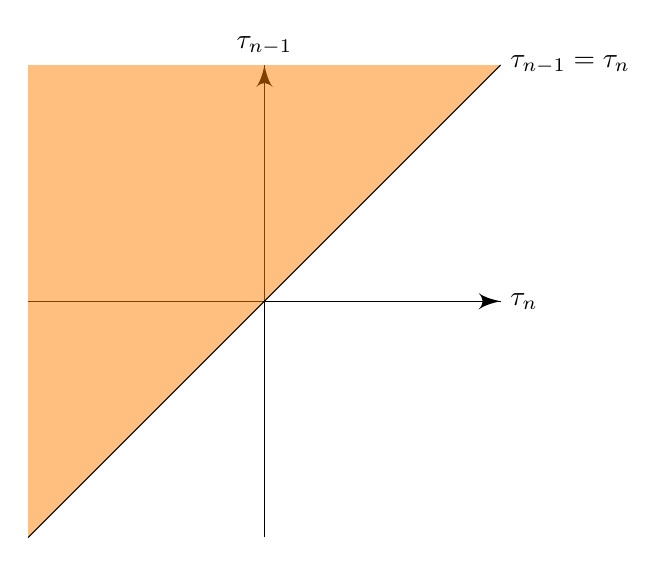
\begin{tikzpicture}
      \draw [->] (-3, 0) -- (3, 0) node [right] {$\tau_n$};
      \draw [->] (0, -3) -- (0, 3) node [above] {$\tau_{n - 1}$};

      \fill [opacity=0.5, morange] (-3, -3) -- (3, 3) -- (-3, 3) -- cycle;
      \draw (-3, -3) -- (3, 3) node [right] {$\tau_{n - 1} = \tau_n$};
    \end{tikzpicture}
  \end{center}
  So we find that
  \[
    S_T = \sum_n (+i)^n \int_{-\infty}^\infty \d \tau_1 \int_{-\infty}^{\tau_1} \d \tau_2 \cdots \int_{-\infty}^{\tau_{n - 1}} V(\tau_n) V(\tau_{n - 1}) \cdots V(\tau_1).
  \]
  We can then see that this is equal to $S^\dagger$.

  What does this tell us? Consider states $\bket{\eta}$ and $\bket{\xi}$ with
  \begin{align*}
    \bket{\eta_T} &= \hat{T} \bket{\eta}\\
    \bket{\xi_T} &= \hat{T} \bket{\xi}
  \end{align*}
  The Dirac bra-ket notation isn't very useful when we have anti-linear operators. So we will write inner products explicitly. We have
  \begin{align*}
    (\eta_T, S\xi_T) &= (\hat{T} \eta, S\hat{T} \xi) \\
    &= (\hat{T} \eta, S_T^\dagger \hat{T} \xi) \\
    &= (\hat{T} \eta, \hat{T} S^\dagger, \xi) \\
    &= (\eta, S^\dagger \xi)^* \\
    &= (\xi, S\eta)
  \end{align*}
  where we used the fact that $\hat{T}$ is anti-unitary. So the conclusion is
  \[
    \brak{\eta_T} S\bket{\xi_T} = \brak{\xi}S\bket{\eta}.
  \]
  So if
  \[
    \hat{T} \mathcal{L}_I(x) \hat{T}^{-1} = \mathcal{L}_I(x_T),
  \]
  then the $S$-matrix elements are equal for time-reversed processes, where the initial and final states are swapped.
\end{eg}

\subsection{CPT theorem}
\begin{thm}[CPT theorem]\index{CPT theorem}
  Any Lorentz invariant Lagrangian with a Hermitian Hamiltonian should be invariant under the product of P, C and T.
\end{thm}
We will not prove this. For details, one can read Streater and Wightman, \emph{PCT, spin and statistics and all that} (1989).

All observations we make suggest that CPT is respected in nature. This means a particle propagating forwards in time cannot be distinguished from the antiparticle propagating backwards in time.

\subsection{Baryogenesis}
In the universe, we observe that there is much more matter than anti-matter. \emph{Baryogenesis}\index{baryogenesis} is the generation of this asymmetry in the universe. Sakarhov came up with three conditions that are necessary for this to happen.
\begin{enumerate}
  \item Baryon number violation (or leptogenesis, ie. lepton number asymmetry), ie. some process $X \to Y + B$ that generates an excess baryon.
  \item Non-equilibrium. Otherwise, the rate of $Y + B \to X$ is the same as the rate of $X \to Y + B$.
  \item C and CP violation. Otherwise, the rate of $X \to Y + B$ and the rate of $\bar{X} \to \bar{Y} + \bar{B}$ would be the same, and the effects cancel out each other.

    We similarly need CP violation, or else the rate of $X \to nq_L$ and the rate of $X \to n q_R$, where $q_{L, R}$ are left and right handed quarks, is equal to the rate of $\bar{x} \to n \bar{q}_L$ and $\bar{x} \to n\bar{q}_R$, and this will wash out our excess.
\end{enumerate}

\section{Spontaneous symmetry breaking}
In this chapter, we are going to look at spontaneous symmetry breaking. The general setting is as follows --- our Lagrangian $\mathcal{L}$ enjoys some symmetry. However, the potential has \emph{multiple} minima. Usually, in perturbation theory, we imagine we are sitting near an equilibrium point of the system (the ``vacuum''), and then look at what happens to small perturbations near the equilibrium.

When there are multiple minima, we have to arbitrarily pick a minimum to be our vacuum, and then do perturbation around it. In many cases, this choice of minimum is \emph{not} invariant under our symmetries. Thus, even though the theory itself is symmetric, the symmetry is lost once we pick a vacuum. It turns out interesting things happen when this happens.

\subsection{Discrete symmetry}
We first consider the case of a discrete symmetry. Consider a real scalar field $\phi(x)$ with a symmetric potential $V(\phi)$, so that
\[
  V(-\phi) = V(\phi).
\]
This gives a discrete ($\Z/2$) symmetry $\phi \leftrightarrow -\phi$.

We will consider the case of a $\phi^4$ theory, with Lagrangian
\[
  \mathcal{L} = \frac{1}{2} \partial_\mu \phi \partial^\mu \phi - \left(\frac{1}{2} m^2 \phi^2 - \frac{\lambda}{4!} \phi^4\right)
\]
for some $\lambda$.

We want the potential to $\to \infty$ as $\phi \to \infty$, so we necessarily require $\lambda > 0$. However, since the $\phi^4$ term dominates for large $\phi$, We are now free to pick the sign of $m^2$, and still get a sensible theory.

Usually, this theory has $m^2 > 0$, and thus $V(\phi)$ has a minimum at $\phi = 0$:
\begin{center}
  \begin{tikzpicture}
    \draw [->](-3, 0) -- (3, 0) node [right] {$\phi$};
    \draw [->] (0, -1.2) -- (0, 3) node [above] {$S(\phi)$};

    \draw [mblue, thick, domain=-1.414:1.414, samples=50] plot [smooth] (\x, {4 * ((\x/2)^4 + (\x/2)^2)});
  \end{tikzpicture}
\end{center}
However, we could imagine a scenario where $m^2 < 0$. In this case, the potential looks like
\begin{center}
  \begin{tikzpicture}
    \draw [->](-3, 0) -- (3, 0) node [right] {$\phi$};
    \draw [->] (0, -1.2) -- (0, 3) node [above] {$V(\phi)$};

    \draw [mblue, thick, domain=-2.4:2.4, samples=50] plot [smooth] (\x, {4 * ((\x/2)^4 - (\x/2)^2)});

    \draw [dashed] (1.414, 0) node [above] {$v$} -- (1.414, -1);
  \end{tikzpicture}
\end{center}
To understand this potential better, we complete the square, and write it as
\[
  V(\phi) = \frac{\lambda}{4} (\phi^2 - v^2)^2 + \text{constant},
\]
where
\[
  v = \sqrt{-\frac{m^2}{\lambda}}.
\]
We see that now $\phi = 0$ become a local maximum, and there are two (global) minima at $\phi = \pm v$. In particular, $\phi$ has acquired a non-zero \term{vacuum expectation value} (\term{VEV}).

We shall wlog consider small excitations around $\phi = v$. Let's write
\[
  \phi(x) = v + cf(x).
\]
Then we can write the Lagrangian as
\[
  \mathcal{L} = \frac{1}{2} \partial_\mu f \partial^\mu f - \lambda \left(v^2 f^2 + + vf^3 + \frac{1}{4} f^4\right),
\]
plus some constants. Therefore $f$ is a scalar field with mass
\[
  m_f^2 = 2v^2 \lambda.
\]
This $\mathcal{L}$ is \emph{not} invariant under $f \to -f$. The symmetry of the original Lagrangian has been broken by the VEV of $\phi$.

\subsection{Continuous symmetry}
We can consider a slight generalization of the above scenario. Consider an $n$-component real scalar field $\phi = (\phi_1, \phi_2, \cdots, \phi_N)^T$, with Lagrangian
\[
  \mathcal{L} = \frac{1}{2} (\partial^\mu \phi) \cdot (\partial_\mu \phi) - V(\phi),
\]
where
\[
  V(\phi) = \frac{1}{2} m^2 \phi^2 + \frac{\lambda}{4} \phi^4.
\]
As before, we will require that $\lambda > 0$.

This is a theory that is invariant under global $\Or(N)$ transforms of $\phi$. Again, if $m^2 > 0$, then $\phi = 0$ is a global minimum, and we do not have spontaneous symmetry breaking. Thus, we consider the case $m^2 < 0$.

In this case, we can write
\[
  V(\phi) = \frac{\lambda}{4} (\phi^2 - v^2)^2 + \text{constant},
\]
where
\[
  v = -\frac{m^2}{\lambda} > 0.
\]
So \emph{any} $\phi$ with $\phi^2 = v^2$ gives a global minimum of the system, and so we have a continuum of vacua. We call this a \term{Sombrero potential} (or \term{wine bottle potential}).
% include sketch

Without loss of generality, we may choose the vacuum to be
\[
  \phi_0 = (0, 0, \cdots, 0, v)^T.
\]
We can then consider steady small fluctuations about this:
\[
  \phi(x) = (\pi_1(x), \pi_2(x), \cdots, \pi_{N-1}(x), v + \sigma(x))^T.
\]
We now have a $\pi$ field with $N - 1$ components, plus a $1$-component $\sigma$ field.

We rewrite the Lagrangian in terms of the $\pi$ and $\sigma$ fields as
\[
  \mathcal{L} = \frac{1}{2}(\partial^\mu \pi) \cdot (\partial_\mu \pi) + \frac{1}{2}(\partial^\mu \sigma) \cdot (\partial_\mu \sigma) - V(\pi, \sigma),
\]
where
\[
  V(\pi, \sigma) = \frac{1}{2} m_\sigma^2 \sigma^s + \lambda v(\sigma^2 + \pi^2) \sigma + \frac{\lambda}{4}(\sigma^2 + \pi^2)^2.
\]
Again, we have dropped a constant term.

In this Lagrangian, we see that the $\sigma$ field has mass
\[
  m_\sigma = \sqrt{2\lambda v^2},
\]
but the $\pi$ fields are massless. We can understand this as follows --- the $\sigma$ field corresponds to the radial direction in the potential, and this is locally quadratic, and hence has a mass term. However, the $\pi$ fields correspond to the excitations in the azimuthal directions, which are flat.

\subsection{General case}
What we just saw is a completely general phenomenon. Suppose we have an $N$-dimensional field $\phi = (\phi_1, \cdots, \phi_N)$, and suppose our theory has a Lie group of symmetries $G$. We will assume that the action of $G$ preserves the potential and kinetic terms individually, and not just the Lagrangian as a whole, so that $G$ will send a vacuum to another vacuum.

Suppose there is more than one choice of vacuum. We write
\[
  \Phi_0 = \{\phi_0: V(\phi_0) = V_{\mathrm{min}}\}
\]
for the set of all vacua. Now we pick a favorite vacuum $\phi_0 \in \Phi_0$, and we want to look at the elements of $G$ that fixes this vacuum. We write
\[
  H = \stab(\phi_0) = \{h \in G: h \phi_0 = \phi_0\}.
\]
This is the \term{invariant subgroup}, or \term{stabilizer subgroup} of $\phi_0$. This is the symmetry we are left with after the spontaneous symmetry breaking.

We will make some further simplifying assumptions. We will suppose $G$ acts \emph{transitively} on $\Phi_0$, ie. given any two vacua $\phi_0, \phi_0'$, we can find some $g \in G$ such that
\[
  \phi_0' = g \phi_0.
\]
This ensures that any two vacua are ``the same'', so which $\phi_0$ we pick doesn't really matter. Indeed, given two such vacua and $g$ relating them, it is a straightforward computation to check that
\[
  \stab(\phi_0') = g \stab(\phi_0) g^{-1}.
\]
So any two choices of vacuum will result in conjugate, and in particular isomorphic, subgroups $H$.

It is a curious, and also unimportant, observation that we given a choice of vacuum $\phi_0$, we have a canonical bijection
\[
  \begin{tikzcd}[cdmap]
    G/H \ar[r, "\sim"] & \Phi_0\\
    g \ar[r, maps to] & g \phi_0
  \end{tikzcd}.
\]
So we can identify $G/H$ and $\Phi_0$.

We now try to understand what happens when we try to do perturbation theory around our choice of vacuum. At $\phi = \phi_0 + \delta \phi$, we can as usual write
\[
  V(\phi_0 + \delta \phi) - V(\phi_0) = \frac{1}{2} \delta \phi_r \frac{\partial^2 V}{\partial \phi_r \partial \phi_s} \delta \phi_s + O(\delta \phi^3).
\]
This quadratic $\partial^2 V$ term is now acting as a mass. We call it the \term{mass matrix}
\[
  M_{rs}^2 = \frac{\partial^2 V}{\partial \phi_r \partial \phi_s}.
\]
Note that we are being sloppy with where our indices go, because $(M^2)^{rs}$ is ugly. It doesn't really matter much, since $\phi$ takes values in $\R^N$ (or $\C^n$), which is a Euclidean space.

In our previous example, we saw that there were certain modes that went massless. We now want to see if the same happens. To do so, we pick a basis $\{\tilde{t}^a\}$ of $\mathfrak{h}$ (the Lie algebra of $H$), and then extend it to a basis $\{t^a, \theta^a\}$ of $\mathfrak{g}$.

We consider a variation
\[
  \delta \phi = \varepsilon \theta^a \phi_0
\]
around $\phi_0$.

Note that when we write $\theta^a \phi_0$, we mean the resulting infinitesimal change of $\phi_0$ when $\theta^a$ acts on field. For a general Lie algebra element, this may be zero. However, we know that $\theta^a$ does not belong to $\mathfrak{h}$, so it does not fix $\phi_0$. Thus (assuming sensible non-degeneracy conditions) this implies that $\theta^a \phi_0$ is non-zero.

At this point, the uncareful reader might be tempted to say that since $G$ is a symmetry of $V$, we must have $V(\phi_0 + \delta \phi) = V(\phi_0)$, and thus
\[
  (\theta^a \phi)_r M_{rs}^2 (\theta^a \phi)_s = 0,
\]
and so we have found zero eigenvectors of $M_{rs}$. But this is wrong. For example, if we take
\[
  M =
  \begin{pmatrix}
    1 & 0\\
    0 & -1
  \end{pmatrix},\quad
  \theta^a \phi =
  \begin{pmatrix}
    1\\1
  \end{pmatrix},
\]
then our previous equation holds, but $\theta^a \phi$ is \emph{not} a zero eigenvector. We need to be a bit more careful.

Instead, we note that by definition of $G$-invariance, for any field value $\phi$ and a corresponding variation
\[
  \phi \mapsto \phi + \varepsilon \theta^a \phi,
\]
we must have
\[
  V(\phi + \delta \phi) = V(\phi),
\]
since this is what it means for $G$ to be a symmetry.

Expanding to first order, this says
\[
  V(\phi + \delta \phi) - V(\phi) = \varepsilon (\theta^a \phi)_r \frac{\partial V}{\partial \phi_r} = 0.
\]
Now the trick is to take a further derivative of this. We obtain
\[
  0 = \frac{\partial}{\partial \phi_s} \left((\theta^a \phi)_r \frac{\partial V}{\partial \phi_r}\right) = \left(\frac{\partial}{\partial \phi_s} (\theta^a \phi)_r\right) \frac{\partial V}{\partial \phi_r} + (\theta^a \phi)_r M_{rs}^2.
\]
Now at a vacuum $\phi = \phi_0$, the first term vanishes. So we must have
\[
  (\theta^a \phi_0)_r M_{rs}^2 = 0.
\]
By assumption, $\theta^a \phi_0 \not= 0$. So we have found a zero vector of $M_{rs}$. Recall that we had $\dim G - \dim H$ of these $\theta^a$ in total. So we have found $\dim G - \dim H$ zero eigenvectors in total.

We can do a small sanity check. What if we replaced $\theta^a$ with $t^a$? The same derivations would still follow through, and we deduce that
\[
  (t^a \phi_0)_r M_{rs}^2 = 0.
\]
But since $t^a$ is an \emph{unbroken symmetry}, we actually just have $t^a \phi_0 = 0$, and this really doesn't say anything interesting.

What about the other eigenvalues? They could be zero for some other reason, and there is no reason to believe one way or the other. However, generally, in the scenarios we meet, they are usually massive. So after spontaneous symmetry breaking, we end up with $\dim G - \dim H$ massless modes, and $N - (\dim G - \dim H)$ massive ones.

This is \term{Goldstone's theorem} in the classical case.
\begin{eg}
  In our previous $O(N)$ model, we had $G = O(N)$, and $H = O(N - 1)$. These have dimensions
  \[
    \dim G = \frac{N(N - 1)}{2},\quad \dim H = \frac{(N - 1)(N - 2)}{2}.
  \]
  Then we have
  \[
    \Phi_0 \cong S^{N - 1},
  \]
  the $(N - 1)$-dimensional sphere. So we expect to have
  \[
    \frac{N - 1}{2} (N - (N - 2)) = N - 1
  \]
  massless modes, which are the $\pi$ fields we found. We also found $N - (N - 1) = 1$ massive mode, namely the $\sigma$ field.
\end{eg}

\begin{eg}
  In the first discrete case, we had $G = \Z/2\Z$ and $H = \{e\}$. These are (rather degenerate) $0$-dimensional Lie groups. So we expect $0 - 0 = 0$ massless modes, and $1 - 0 = 1$ massive modes, which is what we found.
\end{eg}
\subsection{Goldstone's theorem}
We now consider the quantum version of Goldstone's theorem. We hope to get something similar.

Again, suppose our Lagrangian has a symmetry group $G$, which is spontaneously broken into $H \leq G$ after picking a preferred vacuum $\bket{0}$. Again, we take a Lie algebra basis $\{t_a, \theta_a\}$ of $\mathfrak{g}$, where $\{t_a\}$ is a basis for $\mathfrak{h}$. Note that we will assume that $a$ runs from $1, \cdots, \dim G$, and we use the first $\dim H$ labels to refer to the $t_a$, and the remaining to label the $\theta_a$, so that the actual basis is
\[
  \{t_1, t_2, \cdots, t_{\dim H}, \theta_{\dim H + 1}, \cdots, \theta_{\dim G}\}.
\]
For aesthetic reasons, this time we put the indices on the generators below.

Now recall, say from AQFT, that these symmetries of the Lagrangian give rise to conserved currents $j_a^\mu(x)$. These in turn give us conserved charges
\[
  Q_a = \int \d^3 x\; j^0_a (x).
\]
Moreover, under the action of the $t^a$ and $\theta^a$, the corresponding change in $\phi$ is given by
\[
  \delta \phi = -[Q^a, \phi].
\]
The fact that the $\theta^a$ break the symmetry of $\brak{0}$ tell us that
\[
  \brak{0}[Q^a, \phi(0)] \bket{0} \not= 0.
\]
Note that the choice of evaluating $\phi$ at $0$ is completely arbitrary, but we have to pick somewhere, and $0$ is easy to write. Writing out the definition of $Q_a$, we know that
\[
  \int \d^3 x\; \brak{0} [j_a^0(x), \phi(0)] \bket{0} \not= 0.
\]
More generally, since the label $^0$ is arbitrary by Lorentz invariance, we are really looking at the relation
\[
  \brak{0} [j_a^\mu (x), \phi(0)] \bket{0} \not= 0,
\]
and writing it in this more Lorentz covariant way makes it easier to work with. The goal is to deduce the existence of massless states from this non-vanishing.

For convenience, we will write this expression as
\[
  X_a^\mu = \brak{0} [j_a^\mu (x), \phi(0)] \bket{0}.
\]
We treat the two terms in the commutator separately. The first term is
\[
  \brak{0} j_a^\mu (x) \phi(0) \bket{0} = \sum_n \brak{0}j_a^\mu (x) \bket{n} \brak{n}\phi(0) \bket{0}.\tag{$*$}
\]
We write $p_n$ for the momentum of $\bket{n}$. We now note that
\[
  j_a^\mu (x) = e^{i\hat{p} \cdot x} j_a^\mu (0) e^{-i\hat{p} \cdot x}.
\]
so that
\[
  \brak{0}j_a^\mu(x) \bket{n} = \brak{0} j_a^\mu(0) \bket{n} e^{-ip_n \cdot x}.
\]
We can use this to do some Fourier transform magic. By direct verification, we can see that $(*)$ is equivalent to
\[
  i \int \frac{\d^4 k}{(2\pi)^3} \rho_a^\mu(k) e^{-ik\cdot x},
\]
where
\[
  i \rho_a^\mu (k) = (2\pi)^3 \sum_n \delta^4(k - p_n)\brak{0}j_a^\mu(0) \bket{n} \brak{n}\phi(0)\bket{0}.
\]
Similarly, we define
\[
  i \tilde{\rho}_a^\mu (k) = (2\pi)^3 \sum_n \delta^4(k - p_n) \brak{0} \phi(0) \bket{n} \brak{n} j_a^\mu (0) \bket{0}.
\]
Then we can write
\[
  X_a^\mu = i \int \frac{\d^4 k}{(2\pi)^3}\left(\rho_a^\mu (k) e^{-ik\cdot x} - \tilde{\rho}_a^\mu(k) e^{+ik\cdot x}\right).
\]
This is called the \term{K\"allen-Lehmann spectral representation}.

We now claim that $\rho_a^\mu(k)$ and $\tilde{\rho}_a^\mu(k)$ can be written in a particularly nice form. This involves a few observations (when I say $\rho_a^\mu$, I actually mean $\rho_a^\mu$ and $\tilde{\rho}_a^\mu$):
\begin{itemize}
  \item $\rho_a^\mu$ depends Lorentz covariantly in $k$. So it ``must'' be a scalar multiple of $k^\mu$.
  \item $\rho_a^\mu(k)$ must vanish when $k^0 > 0$, since $k^0 \leq 0$ is non-physical. % why?
  \item By Lorentz invariance, the magnitude of $\rho_a^\mu(k)$ can depend only on the length (squared) $k^2$ of $k$.
\end{itemize}
Under these assumptions, we can write can write $\rho_a^\mu$ and $\tilde{\rho}_a^\mu$ as
\begin{align*}
  \rho_a^\mu (k) &= k^\mu \Theta(k^0) \rho_a (k^2),\\
  \tilde{\rho}_a^\mu (k) &= k^\mu \Theta(k^0) \tilde{\rho}_a(k^2),
\end{align*}
where $\Theta$ is the \term{Heaviside theta function}
\[
  \Theta(x) =
  \begin{cases}
    1 & x > 0\\
    0 & x \leq 0
  \end{cases}.
\]
So we can write
\[
  X_a^\mu = i \int \frac{\d^4 k}{(2\pi)^3}\;k^\mu \Theta(k^0) (\rho_a(k^2)e^{-ik\cdot x} - \tilde{\rho}_a(k^2) e^{+ik\cdot x}).
\]
We now use the (nasty?) trick of hiding the $k^\mu$ by replacing it with a derivative:
\[
  X_a^\mu = - \partial^\mu \int \frac{\d^4 k}{(2\pi)^3} \Theta(k^0)\left(\rho_a(k^2) e^{-ik\cdot x} + \tilde{\rho}_a(k^2) e^{ik\cdot x}\right).
\]
Now we might find the expression inside the integral a bit familiar. Recall that the propagator is given by
\[
  D(x, \sigma) = \brak{0} \phi(x) \phi(0) \bket{0} = \int \frac{\d^4 k}{(2\pi)^3}\; \Theta(k^0) \delta(k^2 - \sigma) e^{-ik\cdot x}.
\]
where $\sigma$ is the square of the mass of the field. Using the really silly fact that
\[
  \rho_a(k^2) = \int \d \sigma\; \rho_a(\sigma) \delta(k^2 - \sigma),
\]
we find that
\[
  X_a^\mu = -\partial^\mu \int \d \sigma\; (\rho_a(\sigma) D(x, \sigma) + \tilde{\rho}_a (\sigma) D(-x, \sigma)).
\]
Now we have to recall more properties of $D$. For spacelike $x$, we have $D(x, \sigma) = D(-x, \sigma)$. Therefore, requiring $X_a^\mu$ to vanish for spacelike $x$ by causality, we see that we must have
\[
  \rho_a(\sigma) = - \tilde{\rho}_a(\sigma).
\]
Therefore we can write
\[
  X_a^\mu = -\partial^\mu \int \d \sigma\; \rho^a(\sigma) i\Delta(x, \sigma),\tag{$\dagger$}
\]
where
\[
  i \Delta(x, \sigma) = D(x, \sigma) - D(-x, \sigma) = \int \frac{\d^4 k}{(2\pi)^3} \delta(k^2 - \sigma) \varepsilon(k^0) e^{-ik\cdot x},
\]
and
\[
  \varepsilon(k^0) =
  \begin{cases}
    +1 & k^0 > 0\\
    -1 & k^0 < 0
  \end{cases}.
\]
This $\Delta$ is again a different sort of propagator.

We now use current conservation, which tells us
\[
  \partial_\mu j^\mu_a = 0.
\]
So we must have
\[
  \partial_\mu X_a^\mu =- \partial^2 \int \d \sigma\; \rho_a(\sigma) i \Delta(x, \sigma) = 0.
\]
On the other hand, by inspection, we see that $\Delta$ satisfies the Klein-Gordon equation
\[
  (\partial^2 + \sigma) \Delta = 0.
\]
So in $(\dagger)$, we can replace $-\partial^2 \Delta$ with $\sigma \Delta$. So we find that
\[
  \partial_\mu X_a^\mu = \int \d \sigma\; \sigma \rho^a (\sigma) i \Delta(x, \sigma) = 0.
\]
This is true for all $x$. In particular, it is true for timelike $x$ where $\Delta$ is non-zero. So we must have
\[
  \sigma \rho_a(\sigma) = 0.
\]
But we also know that $\rho_a(\sigma)$ cannot be identically zero, because $X_a^\mu$ is not. So the only possible explanation is that
\[
  \rho_a(\sigma) = N_a \delta(\sigma),
\]
where $N_a$ is a dimensionful non-zero constant.

Now we retrieve our definitions of $\rho_a$. Recall that they are defined by
\begin{align*}
  i \rho_a^\mu (k) &= (2\pi)^3 \sum_n \delta^4(k - p_n)\brak{0}j_a^\mu(0) \bket{n} \brak{n}\phi(0)\bket{0}\\
  \rho_a^\mu (k) &= k^\mu \Theta(k^0) \rho_a (k^2).
\end{align*}
So the fact that $\rho_a(\sigma) = N_a \delta(\sigma)$ implies that there must be some states, which we shall call $\bket{B(p)}$, of momentum $p$, such that $p^2 = 0$, and
\begin{align*}
  \brak{0}j_a^\mu(0)\bket{B(p)} &\not= 0\\
  \brak{B(p)} \phi(0) \bket{0} &\not= 0.
\end{align*}
The condition that $p^2 = 0$ tell us these particles are massless, which are those massless modes we were looking for! These are the \term{Goldstone bosons}.

We can write the values of the above as
\begin{align*}
  \brak{0} j_a^\mu (0)\bket{B(p)} &= i F_a^B p^\mu\\
  \brak{B(p)} \phi(0)\bket{0} &= Z^B,
\end{align*}
whose form we deduced by Lorentz in/covariance. By dimensional analysis, we know $F_{aB}$ is a dimension $-1$ constant, and $Z_B$ is a dimensionless constant.

From these formulas, we note that since $\phi(0)\bket{0}$ is rotationally invariant, we deduce that $\bket{B(p)}$ also is. So we deduce that these are in fact spin $0$ particles.

Finally, we end with some computations that relate these different numbers we obtained. We will leave the computational details for the reader, and just outline what we should do. Using our formula for $\rho$, we find that
\[
  \brak{0} [j_a^\mu(x), \phi(0)] \bket{0} = - \partial^\mu \int N^a \delta (\sigma) i \Delta(x, \sigma) \;\d \sigma = -iN^a \partial^\mu \Delta(x, 0).
\]
Integrating over space, we find
\[
  \brak{0}[Q_a, \phi(0)]\bket{0} = - iN_a \int \d^3 x\; \partial^0 \Delta(x, 0) = i N_a.
\]
Then we have
\[
  \brak{0} t_a \phi(0)\bket{0} = i \brak{0} [Q_a, \phi(0)]\bket{0} = i \cdot i N_a = -N_a.
\]
So this number $N_a$ sort-of measures how much the symmetry is broken, and we once again see that it is the breaking of symmetry that gives rise to a non-zero $N_a$, hence the massless bosons.

We also recall that we had
\[
  i k^\mu \Theta(k^0) N_a \delta(k^2) = \sum_B \int \frac{\d^3 p}{2|\mathbf{p}|}\; \delta^4(k - p) \brak{0} j_a^\mu(0) \bket{B(p)} \brak{B(p)} \phi(0) \bket{0}.
\]
On the RHS, we can plug in the names we gave for the matrix elements, and on the left, we can write it as an integral
\[
  \int \frac{\d^3 p}{2|\mathbf{p}|} \delta^4 (k - p) i k^\mu N_a = \int \frac{\d^3 p}{2|\mathbf{p}|} \delta^4(k - p) i p^\mu \sum_B F_a^B Z^B.
\]
So we must have
\[
  N^a = \sum_B F_a^B Z^B.
\]
Now for each independent symmetry-breaking $\theta^a \in \mathfrak{g} \setminus \mathfrak{h}$, we obtain a Goldstone boson this way. So all together, we find
\[
  n = \dim G - \dim H
\]
many Goldstone bosons.

%The number of broken generators is
%\[
% n = \dim G - \dim H.
%\]
%So we see that there are $n$ of the $\rho^a$ that have non-zero contributions at $\sigma = 0$.
%
%Here $F_{aB}$ is a rank $n$ matrix, and this gives rise to $n$ Goldstone bosons $B$.

It is important to figure out the assumptions we used to derive the result. We mentioned ``Lorentz invariance'' many times in the proof, so we certainly need to assume our theory is Lorentz invariant. While it may not seem obvious, the proof actually requires there are more than $2$ spacetime dimensions, and in fact the result does not hold in $2$ or $1$ dimensions. Another perhaps subtle point is that we also needed states to have a positive definite norm. % revisit

It turns out in the case of gauge theory, these do not necessarily hold, and we need to work with them separately.

%Note that we assumed we have a Lorentz invariant theory, and we also assumed there were more than $2$ spacetime dimensions. We don't get spontaneous symmetry breaking in $2$ or $1$ dimensions. We also assumed that states have a positive definite norm. % something about things cancelling.


%We now consider spontaneous symmetry breaking in a fully quantum way. Again, the symmetry group $G$ of the Lagrangian is broken spontaneously to $H \leq G$. In other words, the scalar field gets a non-zero vacuum expectation value
%\[
% \brak{0} \phi(x) \bket{0} = \phi_0 \not= 0.
%\]
%The VEV is invariant under $h \in H$, and so
%\[
% \brak{0} h \phi(x) \bket{0} = \phi_0,
%\]
%but this is not invariant under a general $g \in G \setminus H$. Again suppose we have a basis
%\[
% t^a = \{\tilde{t}^i, \tilde{\theta}^{\tilde{a}}\}
%\]
%of $\mathfrak{g}$, where $\tilde{t}^i$ span $\mathfrak{h} \leq \mathfrak{g}$.
%
%Since $G$ is a symmetry of the Lagrangian, we know there are conserved currents and charges, say $j_a^\mu (x)$ and
%\[
% Q_a = \int \d^3 x\; j^0_a = \int \d^3 x\; \pi(x) t_a \phi,
%\]
%where $\pi$ is the conjugate field. Using the canonical commutation relations, we have
%\[
% \delta \phi(0) = i \alpha^a t^a \phi(0) = - [Q^a, \phi(0)] \alpha^a.
%\]
%Thus these charges induce a representation on the Lie algebra of $\phi$. % ???
%
%To investigate excitations from spontaneous symmetry breaking, consider the VEV of
%\[
% X_a^\mu = \brak{0}[j_a^\mu (x), \phi(0)]\bket{0} = \sum_n \left( \brak{0}j_a^\mu (x) \bket{n} \brak{n}\phi(0) \bket{0} - \brak{0}\phi(0) \bket{n} \brak{n}j_a^\mu(x) \bket{0}\right).
%\]
%We can then write this as
%\[
% i \int \frac{\d^4 k}{(2\pi)^3}\left(\rho_a^\mu (k) e^{-ik\cdot x} - \tilde{\rho}_a^\mu(k) e^{+ik\cdot x}\right),
%\]
%where
%\begin{align*}
% i \rho_a^\mu (k) &= (2\pi)^3 \sum_n \delta^4(k - p_n)\brak{0}j_a^\mu(0) \bket{n} \brak{n}\phi(0)\bket{0}\\
% i \tilde{\rho}_a^\mu (k) &= (2\pi)^3 \sum_n \delta^4(k - p_n) \brak{0} \phi(0) \bket{n} \brak{n} j_a^\mu (0) \bket{0}
%\end{align*}
%Note that we had $j_a^\mu(0)$ because the $e^{-ik\cdot x}$ factors generated the translations. Here $p_n$ is the $4$-momentum of $n$. % ???
%This is called the \term{K\"allen-Lehmann spectral representation}.
%
%From the Lorentz covariance of $\rho_a^\mu$ and $\tilde{\rho}_a^\mu$, they must be proportional to $k^\mu$, as that is the only $4$-vector we have that they can be proportional to. % huh?
%
%Physical states have $k^0 > 0$. Then we can write
%\[
% \rho_a^\mu (k) = k^\mu \Theta(k^0) \rho_a (k^2), % This is k squared.
%\]
%where $\Theta$ is the Heaviside function. Similarly, we have
%\[
% \tilde{\rho}_a^\mu (k) = k^\mu \Theta(k^0) \tilde{\rho}_a(k^2).
%\]
%Then we have
%\[
% X_a^\mu = - \partial^\mu \int \frac{\d^4 k}{(2\pi)^3} \Theta(k^0)\left(\rho_a(k^2) e^{-ik\cdot x} + \tilde{\rho}_a(k^2) e^{ik\cdot x}\right).
%\]
%We can try to relate this to the propagator,
%\[
% D(z - y, \sigma) = \brak{0} \phi(x) \phi(y) \bket{0}, % should be phi(z)
%\]
%where $\sigma$ is the square of the mass of the field. We can write this as
%\[
% D(z - y, \sigma) = \int \frac{\d^4 p}{(2\pi)^3} \Theta(p^0) \delta(p^4 - \sigma) e^{-ip\cdot (z - y)}. % what is p^4?
%\]
%Then we can write
%\[
% X_a^\mu = -\partial_\mu \int \d \sigma (\rho_a(\sigma) D(x, \sigma) + \tilde{\rho}_a (\sigma) D(-x, \sigma)).
%\]
%Here we used the fact that
%\[
% \rho(k^2) = \int \d \sigma\; \rho(\sigma) \delta(k^2 - \sigma).
%\]
%Now for spacelike $x$, we have $D(x, \sigma) = D(-x, \sigma)$. Therefore, requiring $X_a^\mu$ to vanish for spacelike $x$ by causality, we see that
%\[
% \rho_a(\sigma) = - \tilde{\rho}_a(\sigma).
%\]
%Therefore we can write
%\[
% X_a^\mu = -\partial^\mu \int \d \sigma\; \rho^a(\sigma) i\Delta(x, \sigma),\tag{$\dagger$}
%\]
%where
%\[
% i \Delta(x, \sigma) = D(x, \sigma) - D(-x, \sigma) = \int \frac{\d^4 k}{(2\pi)^3} \delta(k^2 - \sigma) \varepsilon(k^0) e^{-ik\cdot x},
%\]
%where
%\[
% \varepsilon(k^0) =
% \begin{cases}
% +1 & k^0 > 0\\
% -1 & k^0 < 0
% \end{cases}.
%\]
%We can think of this as some different sort of propagator. For spacelike $x$, this vanishes.
%
%We now use current conservation, so
%\[
% \partial_\mu j^\mu_a = 0.
%\]
%So we find
%\[
% \partial_\mu X_a^\mu =- \partial^2 \int \d \sigma\; \rho_a(\sigma) i \Delta(x, \sigma) = 0.
%\]
%Also, the Klein-Gordon equation gives
%\[
% (\partial^2 + \sigma) \Delta = 0.
%\]
%So we can replace $-\partial^s \Delta$ with $\sigma \Delta$. So
%\[
% \partial_\mu X_a^\mu = \int \d \sigma\; \sigma \rho^a (\sigma) i \Delta(x, \sigma) = 0.
%\]
%This is true for all $x$. In particular, it is true for timelike $x$ where $\Delta$ is non-zero. So we need
%\[
% \sigma \rho(\sigma) = 0.
%\]
%There are two possibilities:
%\begin{enumerate}
% \item $\rho(\sigma) = 0$. This means
% \[
% \brak{0} [j_a^\mu(x), \phi(0)] \bket{0} = 0.
% \]
% So $t^a$ is an unbroken symmetry, and
% \[
% \brak{0} t^a \phi\bket{0} = 0.
% \]
% \item $\rho^a(\sigma) = N^a \delta(\sigma)$, where $N^a$ is a dimensionful non-zero constant.
%\end{enumerate}
%The first case is boring, so we want to figure out what the consequences of (ii) are. Plugging this into $(\dagger)$, we get
%\[
% \brak{0} [j_a^\mu(x), \phi(0)] \bket{0} = - \partial^\mu \int N^a \delta (\sigma) i \Delta(x, \sigma) \;\d \sigma = -iN^a \partial^\mu \Delta(x, 0).
%\]
%Integrating over time, we find
%\[
% \brak{0}[Q^a, \phi(0)]\bket{0} = - iM^a \int \d^3 x\; \partial^0 \Delta(x, 0) = i N^a.
%\]
%Then we have\[
% \brak{0} t^a \phi_0\bket{0} = i \brak{0} [Q^a, \phi(0)]\bket{0} = i \cdot i N^a = -N^a.
%\]
%Now if $N^a$ and $\phi_0$ are both non-zero, then some states in $\rho_a^\mu$ and $\tilde{\rho}_a^\mu$ have non-zero matrix elements. Label these states by $B(p)$. From Lorentz covariance and dimensional analysis, we have
%\begin{align*}
% \brak{0} j_a^\mu (0)\bket{B(p)} &= i F_{aB} p^\mu\\
% \brak{B(p)} \phi(0)\bket{0} &= Z_B,
%\end{align*}
%where $F_{aB}$ is a dimension $-1$ constant, and $Z_B$ is a dimensionless constnat.
%
%We see that $B(p)$ are spin zero by rotation invariance, and massless (only contribute when $\sigma = p^2 = 0$). We have
%\[
% i \rho_a^\mu (k) = i k^\mu \Theta(k^0) N^a \sigma(k^2) = \sum_B \int \frac{\d^3 p}{2|\mathbf{p}|} \delta^4(k - p) \brak{0} j_a^\mu(0) \bket{B(p)} \brak{B(p)} \phi(0) \bket{0}.
%\]
%We write the LHS as an integral, and plug in the matrix element on the RHS. Then we see that
%\[
% \int \frac{\d^3 p}{2|\mathbf{p}|} \delta^4 (k - p) i k^\mu N^a = \int \frac{\d^3 p}{2|\mathbf{p}|} \delta^4(k - p) i p^\mu \sum_B F_{aB} Z_B.
%\]
%So we have
%\[
% N^a = \sum_B F_{aB} Z_B.
%\]
%The number of broken generators is
%\[
% n = \dim G - \dim H.
%\]
%So we see that there are $n$ of the $\rho^a$ that have non-zero contributions at $\sigma = 0$.
%
%Here $F_{aB}$ is a rank $n$ matrix, and this gives rise to $n$ Goldstone bosons $B$.
%
%Note that we assumed we have a Lorentz invariant theory, and we also assumed there were more than $2$ spacetime dimensions. We don't get spontaneous symmetry breaking in $2$ or $1$ dimensions. We also assumed that states have a positive definite norm. % something about things cancelling.

\subsection{The Higgs mechanism}
Recall that we had a few condition for our previous theorem to hold. In the case of gauge theories, these typically don't hold. For example, in QED, imposing a Lorentz invariant gauge condition (eg. the Lorentz gauge) gives us negative norm states. On the other hand, if we fix the gauge condition so that we don't have negative norm states, this breaks Lorentz invariance. What happens in this case is known as the \term{Higgs mechanism}.

Let's consider the case of scalar electrodynamics. This involves two fields:
\begin{itemize}
  \item A complex scalar field $\phi(x) \in \C$.
  \item A 4-vector field $A(x) \in \R^{1, 3}$.
\end{itemize}
As usual the components of $A(x)$ are denoted $A_\mu(x)$. From this we define the electromagnetic field tensor
\[
  F_{\mu\nu} = \partial_\mu A_\nu - \partial_\nu A_\mu,
\]
and we have a covariant derivative
\[
  \D_\mu = \partial_\mu + i q A_\mu.
\]
As usual, the Lagrangian is given by
\[
  \mathcal{L} = -\frac{1}{4} F_{\mu\nu} F^{\mu\nu} + (\D_\mu \phi)^* (\D^\mu \phi) - V(|\phi|^2)
\]
for some potential $V$.

A $\U(1)$ gauge transformation is specified by some $\alpha(x) \in \R$. Then the fields transform as
\begin{align*}
  \phi(x) &\mapsto e^{i\alpha(x)} \phi(x)\\
  A_\mu(x) &\mapsto A_\mu(x) - \frac{1}{q} \partial_\mu \alpha(x).
\end{align*}
We will consider a $\phi^4$ theory, so that the potential is
\[
  V(|\phi|^2) = \mu^2 |\phi|^2 + \lambda |\phi|^4.
\]
As usual, we require $\lambda > 0$, and if $\mu^2 > 0$, then this is boring with a unique vacuum at $\phi = 0$. In this case, $A_\mu$ is massless and $\phi$ is massive.

If instead $\mu^2 < 0$, then this is the interesting case. We have a minima at
\[
  |\phi_0|^2 = -\frac{\mu^2}{2\lambda} \equiv \frac{v^2}{2}.
\]
Without loss of generality, we expand around a real $\phi_0$, and write
\[
  \phi(x) = \frac{1}{\sqrt{2}} e^{i \theta(x)/v} (v + \eta(x)),
\]
where $\eta, \theta$ are \emph{real} fields.

Now we notice that $\theta$ isn't a ``genuine'' field (despite being real). Our theory is invariant under gauge transformations. Thus, by picking
\[
  \alpha(x) = - \frac{1}{v} \theta(x),
\]
we can get rid of the $\theta(x)$ term, and be left with
\[
  \phi(x) = \frac{1}{\sqrt{2}}(v + \eta(x)).
\]
This is called the \term{unitary gauge}. Of course, once we have made this choice, we no longer have the gauge freedom, but on the other hand everything else going on becomes much clearer.

%For small fluctuations, we approximate
%\[
% \phi(x) \approx \frac{1}{\sqrt{2}} (v + \eta + i \theta).
%\]
%We will chose $v > 0$. We substitute this into the potential to get
%\[
% V(\phi^* \phi) = \lambda \left(|\phi|^2 - \frac{v^2}{2}\right)^2 = \frac{\lambda}{4} (v^2 + \eta^2 + 2 v \eta - v^2)^2
%\]
%where we as usual dropped a constant. Putting this to the Lagrangian, we get
%\[
% \mathcal{L} = \frac{1}{2} \left(\partial_\mu \eta \partial^\mu \eta + 2 \mu^2 \eta^2\right) + \frac{1}{2} \partial_\mu \theta \partial^\mu \theta - \frac{1}{4} F^{\mu\nu} F_{\mu\nu} + qv A_\mu \partial^\mu \theta + \frac{q^2 v^2}{2} A_\mu A^\mu + \mathcal{L}_{\mathrm{int}},
%\]
%where $\mathcal{L}_{\mathrm{int}}$ involves terms with $\geq 2$ fields.
%
%It appears that that we have a mass for $\eta$ and $A_\mu$, but not $\theta$, and also a strange $A_\mu \partial^\mu \theta$ term.
%
%To see what is going on, we transform to the \term{unitary gauge}.
%\[
% A_\mu \mapsto A_\mu + \frac{1}{qv} \partial_\mu \theta(x),
%\]
%where we have chosen
%\[
% \alpha(x) = - \frac{1}{v} \theta(x).
%\]
%Then the $\phi$ field transforms as
%\[
% \phi \mapsto e^{i\theta/v} \phi = \frac{1}{2} (v + \eta).
%\]
%This corresponds to getting rid of the phase, and so we may assume $\phi$ is real.
In this gauge, the Lagrangian can be written as
\[
  \mathcal{L} = \frac{1}{2}(\partial_\mu \eta \partial^\mu \eta + 2 \mu^2 \eta^2) - \frac{1}{4} F^{\mu\nu}F_{\mu\nu} + \frac{q^2 v^2}{2} A_\mu A^\mu + \mathcal{L}_{\mathrm{int}},
\]
where $\mathcal{L}_{\mathrm{int}}$ is the interaction piece that involves more than two fields.

We can now just read off what is going on in here.
\begin{itemize}
  \item The $\eta$ field is massive with mass
    \[
      m_\mu^2 = - 2 \mu^2 = 2 \lambda v^2 > 0.
    \]
  \item The photon now gains a mass
    \[
      m_A^2 = q^2 v^2.
    \]
  \item What would be the Goldstone boson, namely the $\theta$ field, has been ``eaten'' to become the longitudinal polarization of $A_\mu$ and $A_\mu$ has gained a degree of freedom (or rather, the gauge non-degree-of-freedom became a genuine degree of freedom).
\end{itemize}
One can check that the interaction piece becomes
\[
  \mathcal{L}_{\mathrm{int}} = \frac{q^2}{2} A^\mu A^\mu \eta^2 + q m_A A_\mu A^\mu \eta - \frac{\lambda}{4} \eta^4 - m_\eta \sqrt{\frac{\lambda}{2}} \eta^3.
\]
So we have interactions that look like
\begin{center}
  \begin{tikzpicture}
    \begin{feynman}
      \vertex (tl);
      \vertex [below right=of tl] (c);
      \vertex [above right=of c] (tr);
      \vertex [below left=of c] (bl);
      \vertex [below right=of c] (br);

      \diagram*{
        (tl) -- [photon] (c) -- [photon] (tr)
        (bl) -- [scalar] (c) -- [scalar] (br)
      };
    \end{feynman}
  \end{tikzpicture}
  \quad
  \begin{tikzpicture}
    \begin{feynman}
      \vertex (tl);
      \vertex [below right=of tl] (c);
      \vertex [above right=of c] (tr);
      \vertex [below =of c] (b);

      \diagram*{
        (tl) -- [photon] (c) -- [photon] (tr)
        (b) -- [scalar] (c);
      };
    \end{feynman}
  \end{tikzpicture}
  \quad
  \begin{tikzpicture}
    \begin{feynman}
      \vertex (tl);
      \vertex [below right=of tl] (c);
      \vertex [above right=of c] (tr);
      \vertex [below left=of c] (bl);
      \vertex [below right=of c] (br);

      \diagram*{
        (tl) -- [scalar] (c) -- [scalar] (tr)
        (bl) -- [scalar] (c) -- [scalar] (br)
      };
    \end{feynman}
  \end{tikzpicture}
  \quad
  \begin{tikzpicture}
    \begin{feynman}
      \vertex (tl);
      \vertex [below right=of tl] (c);
      \vertex [above right=of c] (tr);
      \vertex [below =of c] (b);

      \diagram*{
        (tl) -- [scalar] (c) -- [scalar] (tr)
        (b) -- [scalar] (c);
      };
    \end{feynman}
  \end{tikzpicture}
\end{center}
This $\eta$ field is the ``Higgs boson'' in our toy theory.

\subsection{Non-abelian theories}
We now quickly write down the general set up of non-abelian gauge theories. We will not go into specific examples or do much about them, as we will soon actually start to discuss the standard model, and see many examples of these.

In general, we have a gauge group $G$, which is a compact Lie group with Lie algebra $\mathfrak{g}$. We also have a representation of $G$ on $\C^n$, which we will assume is unitary, ie. each element of $G$ is represented by a unitary matrix. Our field $\psi(x) \in \C^n$ takes values in this representation.

A \term{gauge transformation} is specified by giving a $g(x) \in G$ for each point $x$ in the universe, and then the field transforms as
\[
  \psi(x) \mapsto g(x) \psi(x).
\]
Alternatively, we can represent this transformation infinitesimally, by producing some $t(x) \in \mathfrak{g}$, and then the transformation is specified by
\[
  \psi(x) \mapsto \exp(i t(x)) \psi(x).
\]
Associated to our gauge theory is a \term{gauge field} $A_\mu(x) \in \mathfrak{g}$ (ie. we have an element of $\mathfrak{g}$ for each $\mu$ and $x$), which transforms under an infinitesimal transformation $t(x) \in \mathfrak{g}$ as
\[
  A_\mu(x) \mapsto - \partial_\mu t(x) + [t, A_\mu].
\]
The gauge covariant derivative is again give by
\[
  \D_\mu = \partial_\mu + i g A_\mu.
\]
where all fields are, of course, implicitly evaluated at $x$. As before, we can define
\[
  F_{\mu\nu} = \partial_\mu A_\nu - \partial_\nu A_\mu - g [A_\mu, A_\nu] \in \mathfrak{g},
\]
Alternatively, we can write this as
\[
  [\D_\mu, \D_\nu] = ig F_{\mu\nu}.
\]
We will later on work in coordinates. We can pick a basis of $\mathfrak{g}$, say $t^1, \cdots, t^n$. Then we can write an arbitrary element of $\mathfrak{g}$ as $\theta^a(x) t^a$. Then in this basis, we write the components of the gauge field as $A_\mu^a$, and similarly the field strength is denoted $F_{\mu\nu}^a$. We can define the \term{structure constants} \term{$f^{abc}$} by
\[
  [t^a, t^b] = f^{abc}t^c.
\]
Using this notation, the gauge part of the Lagrangian $\mathcal{L}$ is
\[
  \mathcal{L}_g = -\frac{1}{4} F_{\mu\nu}^a F^{a\mu\nu} = - \frac{1}{2} \Tr (F_{\mu\nu} F^{\mu\nu}). % check
\]
We now move on to look at some actual theories.

\section{Electroweak theory}
The electroweak theory has a gauge group of $\SU(2)_L \times \U(1)_Y$, and also a complex scalar \term{Higgs field} $\phi(x) \in \C^2$. Note that when we say ``scalar'', we mean it doesn't transform under Lorentz transformations (ie. it is not a \emph{tangent} (or cotangent) vector). It is still a ``vector'' in the sense that it has two components.

We will couple these fields to different fermions, namely leptons and quarks, which are Dirac spinor fields.

\subsection{Electroweak gauge theory}
We start by understanding the gauge and Higgs part of the theory. As mentioned, the gauge group is $\SU(2)_L \times \U(1)_Y$. We will see that this is broken by the Higgs mechanism.

It is convenient to pick a basis for $\su(2)$, which we will denote by
\[
  \tau^a = \frac{\sigma^a}{2}.
\]
Note that these are not genuinely elements of $\su(2)$. We need to multiply these by $i$ to actually get members of $\su(2)$. As we will later see, these act on fields as $e^{i \tau^a}$ instead of $e^{\tau^a}$. Under this basis, the structure constants are $f^{abc} = \varepsilon^{abc}$.

We start by describing how our gauge group acts on the Higgs field $\phi(x) \in \C^2$. The $\SU(2)$ part acts in the obvious way, ie. as the fundamental representation. The $\U(1)_Y$ part just acts as complex multiplication, as we saw in electrodynamics theory just now. The field has a \term{hypercharge}, which in our case is $Y = \frac{1}{2}$\index{$Y$}, which we'll see affects how the coupling of $\U(1)_Y$ behaves.

An (infinitesimal) gauge transformation can be represented by elements $\alpha^a(x), \beta(x) \in \R$, corresponding to the elements $\alpha^a(x) \tau^a \in \su(2)$ and $\beta(x) \in \uu (1) \cong \R$. Then the Higgs field transform as
\[
  \phi(x) \mapsto e^{i \alpha^a(x) \tau^a} e^{i \frac{1}{2} \beta(x)} \phi(x),
\]
where the $\frac{1}{2}$ factor of $\beta(x)$ comes from the hypercharge being $\frac{1}{2}$.

The gauge fields corresponding to $\SU(2)$ and $\U(1)$ are denoted $W_\mu^a$ and $B_\mu$, where again $a$ runs through $a = 1, 2, 3$. The covariant derivative associated to these gauge fields is
\[
  \D_\mu = \partial_\mu + i g W_\mu^a \tau^a + \frac{1}{2} g' B_\mu
\]
for some coupling constants $g$ and $g'$.

The part of the Lagrangian relating the gauge and Higgs field is
\[
  \mathcal{L}_{\mathrm{gauge}, \phi} = -\frac{1}{2} \Tr (F^W_{\mu\nu} F^{W,\mu\nu}) - \frac{1}{4} F_{\mu\nu}^B F^{B, \mu\nu} + (\D_\mu \phi)^\dagger (\D^\mu \phi) - \mu^2 |\phi|^2 - \lambda |\phi|^4,
\]
where the field strengths of $W$ and $B$ respectively are given by
\begin{align*}
  F_{\mu\nu}^{W, a} &= \partial_\mu W_\nu^a - \partial_\nu W_\mu^a - g \varepsilon^{abc} W_\mu^b W_\nu^c\\
  F_{\mu\nu}^B &= \partial_\mu B_\nu - \partial_\nu V_\mu.
\end{align*}
In the case $\mu^2 < 0$, the Higgs field acquires a VEV, and we wlog shall choose the vacuum to be
\[
  \phi_0 = \frac{1}{\sqrt{2}}
  \begin{pmatrix}
    0\\ v
  \end{pmatrix},
\]
where
\[
  \mu^2 = - \lambda v^2 < 0.
\]
As in the case of $\U(1)$ symmetry breaking, the gauge term gives us new things with mass. After spending hours working out the computations, we find that $(\D_\mu \phi)^\dagger (\D^\mu \phi)$ contains mass terms
\[
  \frac{1}{2} \frac{v^2}{4} \left(g^2 (W^1)^2 + g^2 (W^2)^2 + (-gW^3 + g' B)^2\right).
\]
This suggests we define the following new fields:
\begin{align*}
  W_\mu^{\pm} &= \frac{1}{\sqrt{2}} (W_\mu^1 \mp i W_\mu^2)\\
  \begin{pmatrix}
    Z_\mu^0\\
    A_\mu
  \end{pmatrix} &=
  \begin{pmatrix}
    \cos \theta_W & - \sin \theta_W\\
    \sin \theta_W & \cos \theta_W
  \end{pmatrix}
  \begin{pmatrix}
    W_\mu^3\\
    B_\mu
  \end{pmatrix},
\end{align*}
where we pick $\theta_W$ such that
\[
  \cos \theta_W = \frac{g}{\sqrt{g^2 + g'^2}},\quad \sin \theta_W = \frac{g'}{\sqrt{g^2 + g'^2}}.
\]
This $\theta_W$ is called the \term{Weinberg angle}. Then the mass term above becomes
\[
  \frac{1}{2} \left(\frac{v^2g^2}{4} ((W^+)^2 + (W^-)^2) + \frac{v^2(g^2 + g'^2)}{4} Z^2\right).
\]
Thus, our particles have masses
\begin{align*}
  m_W &= \frac{vg}{2}\\
  m_Z &= \frac{v}{2} \sqrt{g^2 + g'^2}\\
  m_\gamma &= 0,
\end{align*}
where $\gamma$ is the $A_\mu$ particle, which is the photon. Thus, our original $\SU(2) \times \U(1)_Y$ breaks down to a $\U(1)_{EM}$ symmetry. In terms of the Weinberg angle,
\[
  m_W = m_Z \cos \theta_W.
\]
Thus, through the Higgs mechanism, we find that the $W^{\pm}$ and $Z$ bosons gained mass, but the photon does not. This agrees with what we find experimentally. In practice, we find that the masses are
\begin{align*}
  m_W &\approx \SI{80}{\giga\electronvolt}\\
  m_Z &\approx \SI{91}{\giga\electronvolt}\\
  m_\gamma &< \SI{e-18}{\giga\electronvolt}.
\end{align*}
Also, the Higgs boson gets mass, as what we saw previously. It is given by
\[
  m_H = \sqrt{-2 \mu^2} = \sqrt{2 \lambda v^2}.
\]
Note that the Higgs mass depends on the constant $\lambda$, which we haven't seen anywhere else so far. So we can't tell $m_H$ from what we know about $W$ and $Z$. Thus, until the Higgs was discovered recently, we didn't know about the mass of the Higgs boson. We now know that
\[
  m_H \approx \SI{125}{\giga\electronvolt}.
\]
Note that we didn't write out all terms in the Lagrangian, but as we did before, we are going to get $W^{\pm}$, $Z$-Higgs and Higgs-Higgs interactions.

\subsection{Coupling to leptons}
We now look at how gauge bosons couple to matter. In general, for a particle with hypercharge $Y$, the covariant derivative is
\[
  \D_\mu = \partial_\mu + i g W_\mu^a \tau^a + i g' Y B_\mu
\]
In terms of the $W^{\pm}$ and $Z$ bosons, we can write this as
\begin{multline*}
  D_\mu = \partial_\mu + \frac{ig}{\sqrt{2}} (W_\mu^+ \tau^+ + W_\mu^- \tau^-) + \frac{ig Z_\mu}{\cos \theta_W} (\cos^2 \theta_W \tau^3 - \sin^2 \theta_W Y) \\
  + ig \sin \theta_W A_\mu (\tau^3 + Y),
\end{multline*}
where
\[
  \tau^{\pm} = \tau^1 \pm i \tau^2.
\]
By analogy, we interpret the final term $ig \sin \theta_W A_\mu (\tau^3 + Y)$ is the usual coupling with the photon. So we can identify the (magnitude of the) electron charge as
\[
  e = g \sin \theta_W,
\]
while the $\U(1)_{EM}$ charge matrix is
\[
  Q = \U(1)_{EM} = \tau^3 + Y.
\]
If we want to replace all occurrences of the hypercharge $Y$ with $Q$, then we need to note that
\[
  \cos^2 \theta_W \tau^3 - \sin^2 \theta_W Y = \tau^3 - \sin^2 \theta_W Q.
\]
We now introduce the electron field. The electron field is given by a spinor field $e(x)$. We will decompose it as left and right components
\[
  e(x) = e_L(x) + e_R(x).
\]
There is also a neutrino field $\nu_{e_L}(x)$. We will assume that neutrinos are massless, and there are only left-handed neutrinos. We know this is not entirely true, because of neutrinos oscillation, but the mass is very tiny, and this is a very good approximation.

To come up with an actual electroweak theory, we need to specify a representation of $\SU(2) \times \U(1)$. It is convenient to group our particles by handedness:
\[
  R(x) = e_R(x),\quad L(x) =
  \begin{pmatrix}
    \nu_{e_L}(x)\\
    e_L(x)
  \end{pmatrix}.
\]
Here $R(x)$ is a single spinor, while $L(x)$ consists of a \emph{pair}, or ($\SU(2)$) \term{doublet}\index{$\SU(2)$ doublet} of spinors.

We first look at $R(x)$. Experimentally, we find that $W^{\pm}$ only couples to left-handed leptons. So $R(x)$ will have the \emph{trivial representation} of $\SU(2)$. We also know that electrons have charge $Q = -1$. Since $\tau^3$ acts trivially on $R$, we must have
\[
  Q = Y = -1
\]
for the right-handed leptons.

The left-handed particles are more complicated. We will assert that $L$ has the ``fundamental'' representation of $\SU(2)$, by which we mean given a matrix
\[
  g = \begin{pmatrix}
    a & b\\
    -\bar{b} & \bar{a}
  \end{pmatrix}\in \SU(2),
\]
it acts on $L$ as
\[
  g L =
  \begin{pmatrix}
    a & b\\
    - \bar{b} & \bar{a}
  \end{pmatrix}
  \begin{pmatrix}
    \nu_{e_L}\\
    e_L
  \end{pmatrix} =
  \begin{pmatrix}
    a \nu_{e_L} + b e_L\\
    -\bar{b} \nu_{e_L} + \bar{a} e_L
  \end{pmatrix}.
\]
We know the electron has charge $-1$ and the neutrino has charge $0$. So we need
\[
  Q =
  \begin{pmatrix}
    0 & 0 \\
    0 & -1
  \end{pmatrix}.
\]
Since $Q = \tau^3 + Y$, we must have $Y = -\frac{1}{2}$.

Using this notation, the gauge part of the lepton Lagrangian can be written concisely as
\[
  \mathcal{L}_{\mathrm{lepton}}^{EW} = \bar L i \slashed D L + \bar R i \slashed D R.
\]
Note that $\bar{L}$ means we take the transpose of the matrix $L$, viewed as a matrix with two components, and then take the conjugate of each spinor individually, so that
\[
  \bar{L} =
  \begin{pmatrix}
    \bar{\nu}_{e_L}(x) & \bar{e}_L(x)
  \end{pmatrix}.
\]
How about the mass? Recall that it makes sense to deal with left and right-handed fermions separately only if the fermion is massless. A mass term
\[
  m_e (\bar{e}_Le_R + \bar{e}_R e_L)
\]
would be very bad, because our $\SU(2)$ action mixes $e_L$ with $\nu_{e_L}$.

But we do know that the electron has mass. The answer is that the mass is again granted by the spontaneous symmetry breaking of the Higgs boson. Working in unitary gauge, we can write the Higgs boson as
\[
  \phi(x) = \frac{1}{\sqrt{2}}
  \begin{pmatrix}
    0\\
    v + h(x)
  \end{pmatrix},
\]
with $v, h(x) \in \R$.

The lepton-Higgs interactions is given by
\[
  \mathcal{L}_{\mathrm{lept}, \phi} = - \sqrt{2} \lambda_e (\bar L \phi R + \bar R \phi^\dagger L),
\]
where $\lambda_e$ is the \term{Yukawa coupling}. It is helpful to make it more explicit what we mean by this expression. We have
\[
  \bar{L} \phi R =
  \begin{pmatrix}
    \bar{\nu}_{e_L}(x) & \bar{e}_L(x)
  \end{pmatrix}
  \left(
  \frac{1}{\sqrt{2}}
  \begin{pmatrix}
    0\\
    v + h(x)
  \end{pmatrix}
  \right)
  e_R(x) = \frac{1}{\sqrt{2}} (v + h(x)) \bar{e}_L(x) e_R(x).
\]
Similarly, we can write out the second term and obtain
\begin{align*}
  \mathcal{L}_{\mathrm{lept}, \phi} &= - \lambda_e (v + h) (\bar{e}_L e_R + \bar{e}_R e_L)\\
  &= - m_e \bar{e} e - \lambda_e h \bar{e} e,
\end{align*}
where
\[
  m_e = \lambda_e v.
\]
We see that while the interaction term is a priori gauge invariant, once we have spontaneously broken the symmetry, we have magically obtained a mass term $m_e$. The second term in the Lagrangian is the Higgs-fermion coupling. We see that this is proportional to $m_e$. So massive things couple more strongly.

We now return to the fermion-gauge boson interactions. We can write it as
\[
  \mathcal{L}_{\mathrm{lept}}^{EM, \mathrm{int}} = \frac{g}{2\sqrt{2}} (J^\mu W_\mu^+ + J^{\mu\dagger} W_\mu^-) + e J_{EM}^\mu A_\mu + \frac{g}{2 \cos \theta_W} J_n^\mu Z_\mu.
\]
where
\begin{align*}
  J^\mu_{EM} &= - \bar{e} \gamma^\mu e\\
  J^\mu &= \bar{\nu}_{e_L}\gamma^\mu (1 - \gamma^5) e\\
  J^\mu_n &= \frac{1}{2} \left(\bar{\nu}_{e_L} \gamma^\mu (1 - \gamma^5) \nu_{e_L} - \bar{e} \gamma^\mu (1 - \gamma^5 - 4 \sin^2 \theta_w)e\right)
\end{align*}
Note that $J^\mu_{EM}$ has a negative sign because the electron has negative charge. These currents are known as the \term{EM current}, \term{charge weak current} and \term{neutral weak current} respectively.

There is one thing we haven't mentioned so far. We only talked about electrons and neutrinos, but the standard model has three generations of leptons. There are the \term{muon} (\term{$\mu$}) and \term{tau} (\term{$\tau$}), and corresponding left-handed neutrinos. With these in mind, we introduce
\[
  L^1 =
  \begin{pmatrix}
    \nu_{e_L}\\
    e_L
  \end{pmatrix},\quad
  L^2 =
  \begin{pmatrix}
    \nu_{\mu_L}\\
    \mu_L
  \end{pmatrix},\quad
  L^3 =
  \begin{pmatrix}
    \nu_{\tau_L}\\
    \tau_L
  \end{pmatrix}.
\]
\[
  R^1 = e_R,\quad R^2 = \mu_R,\quad R^3 = \tau_R.
\]
These couple and interact in exactly the same way as the electrons, but have heavier mass. It is straightforward to add these into the $\mathcal{L}_{\mathrm{lept}}^{EW, \mathrm{int}}$ term. What is more interesting is the Higgs interaction, which is given by
\[
  \mathcal{L}_{\mathrm{lept}, \phi} = - \sqrt{2} \Big(\lambda^{ij} \bar{L}^i \phi R^j + (\lambda^\dagger)^{ij} \bar{R}^i \phi^\dagger L^j\Big),
\]
where $i$ and $j$ run over the different generations. What's new now is that we have the matrices $\lambda \in M_3(\C)$. These are \emph{not} predicted by the standard model.

This $\lambda$ is just a general matrix, and there is no reason to expect it to be diagonal. However, in some sense, it is always diagonalizable. The key insight is that we contract the two indices $\lambda$ with two \emph{different} kinds of things. It is a general linear algebra fact that for any matrix $\lambda$ at all, we can find some unitary matrices $U$ and $S$ such that
\[
  \lambda = U \Lambda S^\dagger,
\]
where $\Lambda$ is a diagonal matrix with real entries. We can then transform our fields by
\begin{align*}
  L^i &\mapsto U^{ij} L^j\\
  R^i &\mapsto S^{ij} R^j,
\end{align*}
and this diagonalizes $\mathcal{L}_{\mathrm{lept}, \phi}$.

It is also clear that this leaves $\mathcal{L}_{\mathrm{lept}}^{EW}$ invariant, especially if we look at the expression before symmetry breaking. So the mass eigenstates are the same as the ``\term{weak eigenstates}''. This tells us that after diagonalizing, there is no mixing within the different generations.

This is important. It is \emph{not} possible for quarks (or if we have neutrino mass), and mixing \emph{does} occur in these cases.

\subsection{Quarks}
We now move on to study quarks. There are 6 flavours of quarks, coming in three generations:
\begin{center}
  \begin{tabular}{cccc}
    \toprule
    Charge & First generation & Second generation & Third generation\\
    \midrule
    $+\frac{2}{3}$ & Up ($u$) & Charm ($c$) & Top ($t$)\\
    $-\frac{1}{3}$ & Down ($d$) & Strange ($s$) & Bottom ($b$)\\
    \bottomrule
  \end{tabular}
\end{center}
each of which is a spinor.

The right handed fields have trivial $\SU(2)$ representations, and are thus $\SU(2)$ singlets. We write them as
\[
  u_R = \begin{pmatrix} u_R & c_R & t_R\end{pmatrix}
\]
which have $Y = Q = +\frac{2}{3}$, and
\[
  d_R = \begin{pmatrix} d_R & s_R & b_R\end{pmatrix}
\]
which have $Y = Q = -\frac{1}{3}$.

The left-handed fields are in $\SU(2)$ doublets
\[
  Q_L^i =
  \begin{pmatrix}
    u_L^i\\
    d_L^i
  \end{pmatrix} =
  \begin{pmatrix}
    \begin{pmatrix}
      u\\d
    \end{pmatrix}_L &
    \begin{pmatrix}
      c\\
      s
    \end{pmatrix}_L &
    \begin{pmatrix}
      t\\
      b
    \end{pmatrix}_L
  \end{pmatrix}
\]
and these all have $Y = \frac{1}{6}$. Here $i = 1, 2, 3$ labels generations.

The electroweak part of the Lagrangian is again straightforward, given by
\[
  \mathcal{L}_{\mathrm{quark}}^{EW} = \bar{Q}_L i \slashed \D Q_L + \bar{u}_R i \slashed\D u_R + \bar{d}_R i \slashed{D} d_R.
\]
It takes a bit more work to couple these things with $\phi$. We want to do so in a gauge invariant way. To match up the $\SU(2)$ part, we need a term that looks like
\[
  \bar{Q}_L^i \phi,
\]
as both $Q_L$ and $\phi$ have the fundamental representation. Now to have an invariant $\U(1)$ theory, the hypercharges have to add to zero, as under a $\U(1)$ gauge transformation $\beta(x)$, the term transforms as $e^{i\sum Y_i \beta(x) }$. We see that the term
\[
  \bar{Q}_L^i \phi d_R^i
\]
works well. However, coupling $\bar{Q}_L^i$ with $u_R$ is more problematic. $\bar{Q}_L^i$ has hypercharge $-\frac{1}{6}$ and $u_R$ has hypercharge $+\frac{2}{3}$. So we need another term of hypercharge $-\frac{1}{2}$. To do so, we introduce the \term{charge-conjugated $\phi$}\index{$\phi^c$}, defined by
\[
  (\phi^c)^\alpha = \varepsilon^{\alpha\beta} \phi^{* \beta}.
\]
One can check that this transforms with the fundamental $\SU(2)$ representation, and has $Y = -\frac{1}{2}$. Inserting generic coupling coefficients $\lambda_{u, d}^{ij}$, we write the Lagrangian as
\[
  \mathcal{L}_{\mathrm{quark}, \phi} = - \sqrt{2} (\lambda_d^{ij} \bar{Q}_L^i \phi d_R^i + \lambda_u^{ij} \bar{Q}_L^i \phi^c u_R^j + \mathrm{h.c.}).
\]
Here $\text{h.c.}$ means ``hermitian conjugate''.

Let's try to diagonalize this in the same way we diagonalized leptons. We again work in unitary gauge, so that
\[
  \phi(x) = \frac{1}{\sqrt{2}}
  \begin{pmatrix}
    0\\
    v + h(x)
  \end{pmatrix},
\]
Then the above Lagrangian can be written as
\[
  \mathcal{L}_{\mathrm{quark}, \phi} = - (\lambda_d^{ij} \bar{d}_L^i (v + h) d_R^i + \lambda_u^{ij} \bar{u}_L^i (v + h) u_R^j + \mathrm{h.c.}).
\]
We now write
\begin{align*}
  \lambda_u &= U_u \Lambda_u S_u^\dagger\\
  \lambda_d &= U_d \Lambda_d S_d^\dagger,
\end{align*}
where $\Lambda_{u, d}$ are diagonal and $S_{u, d}, U_{u, d}$ are unitary. We can then transform the field in a similar way:
\[
  u_L \mapsto U_u u_L,\quad d_L \mapsto U_d d_L,\quad u_R \mapsto S_u u_R,\quad d_R \mapsto S_d d_R.
\]
and then it is a routine check that this diagonalizes $\mathcal{L}_{\mathrm{quark}, \phi}$. In particular, the mass term looks like
\[
  -\sum_i (m_d^i \bar{d}_L^i d_R^i + m_d^i \bar{u}_L^i u_R^i + \text{h.c.}),
\]
where
\[
  m_q^i = v \Lambda_q^{ii}.
\]
% Let's stop and think about symmetries. In this basis, the $\mathcal{L}_{\mathrm{quark}, \phi}$ bit is invariant under P, C and T. Similarly, $\mathcal{L}_{\mathrm{gauge}, \phi}$ is also invariant under P, C and T.
How does this affect our electroweak interactions? The $\bar{u}_R i \slashed \D u_R$ and $\bar{d}_R i \slashed \D d_R$ are staying fine, but the different components of $\bar{Q}_L$ ``differently''. In particular, the $W_\mu^{\pm}$ piece given by $\bar{Q}_L i \slashed \D Q_L$ is not invariant. That piece, can be explicitly written out as
\[
  \frac{g}{2\sqrt{2}} J^{\pm \mu} W_{\mu}^{\pm},
\]
where
\[
  J^{\mu+} = \bar{u}_L^i \gamma^\mu d_L^i.
\]
Under the basis transformation, this becomes
\[
  \bar{u}_L^i \gamma^\mu (U_u^\dagger U_d)^{ij} d_L^j.
\]
This is not going to be diagonal in general. This leads to \emph{inter-generational} quark couplings. In other words, we have discovered that the mass eigenstates are (in general) not equal to the weak eigenstates.

The mixing is dictated by the \term{Cabibbo--Kabyashi--Maskawa matrix} (\term{CKM matrix})
\[
  V_{CKM} = U^\dagger_u U_d.
\]
Explicitly, we can write
\[
  V_{CKM} =
  \begin{pmatrix}
    V_{ud} & V_{us} & V_{ub}\\
    V_{cd} & V_{cs} & V_{cb}\\
    V_{td} & V_{ts} & V_{tb}
  \end{pmatrix},
\]
where the subscript indicate which two things it mixes. So far, these matrices are not predicted by any theory, and is manually plugged into the model.

However, the entries aren't completely arbitrary. Being the product of two unitary matrices, we know $V_{CKM}$ is a unitary matrix. Moreover, the entries are only uniquely defined up to some choice of phases, and this further cuts down the number of degrees of freedom.

If we only had two generations, then we get what is known as \term{Cabibbo mixing}. A general $2 \times 2$ unitary matrix has $4$ real parameters --- one angle and three phases. However, redefining each of the 4 quark fields with a global $\U(1)$ transformation, we can remove three relative phases (if we change all of them by the same phase, then nothing happens). We can then write this matrix as
\[
  V =
  \begin{pmatrix}
    \cos \theta_c & \sin \theta_c\\
    - \sin \theta_c & \cos \theta_c
  \end{pmatrix},
\]
where $\theta_c$ is the \term{Cabibbo angle}. Experimentally, we have $\sin \theta_c \approx 0.22$. It turns out the reality of this implies that CP is conserved, which is left as an exercise on the example sheet.

In this case, we explicitly have
\[
  J^{\mu\dagger} = \cos \theta_c \bar{u}_L \gamma^\mu d_L + \sin \theta_c \bar{u}_l \gamma^\mu s_L - \sin \theta_c \bar{c}_L \gamma^\mu d_L + \cos \theta_c \bar{c}_L \gamma^\mu s_L.
\]
If the angle is $0$, then we have no mixing between the generations.

With three generations, there are nine parameters. We can think of this as $3$ (Euler) angles and $6$ phases. As before, we can re-define some of the quark fields to get rid of five relative phases. We can then write $V_{CKM}$ in terms of three angles and $1$ phase. In general, this $V_{CKM}$ is not real, and this gives us CP violation. Of course, if it happens that this phase is real, then we do not have CP violation. Unfortunately, experimentally, we figured this is not the case. By the CPT theorem, we thus deduce that T violation happens as well.

\subsection{Neutrino oscillation and mass}
Since around $2000$, we know that the mass eigenstates and weak eigenstates for neutrinos are not equivalent, as neutrinos were found to change from one flavour to another. This implies there is some mixing between different generations of leptons. The analogous mixing matrix is the \term{Pontecorov--Maki--Nakagawa--Sakata matrix}, written $U_{PMNS}$\index{$U_{PMNS}$}.

As of today, we do not really understand what neutrinos actually are, as neutrinos don't interact much, and we don't have enough experimental data. If neutrinos are Dirac fermions, then they behave just like quarks, and we expect CP violation.

However, there is another possibility. Since neutrinos do not have a charge, it is possible that they are their own anti-particles. In other words, they are \term{Majorana fermions}. It turns out this implies that we cannot get rid of that many phases, and we are left with 3 angles and 3 phases. Again, we get CP violation in general.

We consider these cases briefly in turn.

\subsubsection*{Dirac fermions}
If they are Dirac fermions, then we must also get some right-handed neutrinos, which we write as
\[
  N^i = \nu_R^i = (\nu_{eR}, \nu_{\mu R}, \nu_{\tau R}).
\]
Then we modify the Dirac Lagrangian to say
\[
  \mathcal{L}_{\mathrm{lept}, \phi} = -\sqrt{2} (\lambda^{ij} \bar{L}^i \phi R^j + \lambda_\nu^{ij} \bar{L}^i \phi^c N^j + \mathrm{h.c.}).
\]
This is exactly like for quarks. As in quarks, we obtain a mass term.
\[
  - \sum_i m_\nu^i (\bar{\nu}_R^i \nu_L^i + \bar{\nu}_L^i \nu_R^i).
\]
\subsubsection*{Majorana neutrinos}
If neutrinos are their own anti-particles, then, in the language we had at the beginning of the course, we have
\[
  d^s(p) = b^s(p).
\]
%We take the intrinsic c-parity to be $1$, wlog.
Then $\nu(x) = \nu_L(x) + \nu_R(x)$ must satisfy
\[
  \nu^c(x) = C \bar{\nu}_L^T = \nu(x).
\]
Then we see that we must have
\[
  \nu_R(x) = \nu_L^c(x),
\]
and vice versa. So the right-handed neutrino field is not independent of the left-handed field. In this case, the mass term would look like
\[
  -\frac{1}{2} \sum_i m_\nu^i (\bar{\nu}_L^{ic} \nu_L^i + \bar{\nu}_L^i \nu_L^{ic}).
\]
As in the case of leptons, postulating a mass term directly like this breaks gauge invariance. Again, we solve this problem by coupling with the Higgs field. It takes some work to find a working gauge coupling, and it turns out it the simplest thing that works is
\[
  \mathcal{L}_{L, \phi} = -\frac{Y^{ij}}{M} (L^{iT} \phi^c)C (\phi^{cT} L^j) + \mathrm{h.c.}.
\]
This is weird, because it is a dimension $5$ operator. This dimension 5 operator is \emph{non-renormalizable}. This is actually okay, as along as we think of the standard model as an effective field theory, describing physics at some low energy scale.

\subsection{Summary of electroweak theory}
We can do a quick summary of the electroweak theory. We start with the picture before spontaneous symmetry breaking.

The gauge group of this theory is $\SU(2)_L \times \U(1)_Y$, with gauge fields $W_\mu \in \su(2)$ and $B_\mu \in \uu(1)$. The coupling of $\U(1)$ with the particles is specified by a \emph{hypercharge} $Y$, and the $\SU(2)$ couplings will always be trivial or fundamental. The covariant derivative is given by
\[
  \D_\mu = \partial_\mu + i g W_\mu^a \tau^a + \frac{1}{2} g' Y B_\mu,
\]
where $\tau^a$ are the canonical generators of $\su(2)$. The field strengths are given by
\begin{align*}
  F_{\mu\nu}^{W, a} &= \partial_\mu W_\nu^a - \partial_\nu W_\mu^a - g \varepsilon^{abc} W_\mu^b W_\nu^c\\
  F_{\mu\nu}^B &= \partial_\mu B_\nu - \partial_\nu V_\mu.
\end{align*}
The theory contains the scalar \emph{Higgs field} $\phi \in \C^2$, which has hypercharge $Y = \frac{1}{2}$ and the fundamental $\SU(2)$ representation. We also have three generations of matter, given by
\begin{center}
  \begin{tabular}{ccccccc}
    \toprule
    Type & G1 & G2 & G2 & $Q$ & $Y_L$ & $Y_R$\\
    \midrule
    Positive quarks & $u$ & $c$ & $t$ & $+\frac{2}{3}$ & $+\frac{1}{6}$ & $+\frac{2}{3}$ \\
    Negative quarks & $d$ & $s$ & $b$ & $-\frac{1}{3}$ & $+\frac{1}{6}$ & $-\frac{1}{3}$\\
    \midrule
    Leptons ($e, \mu, \tau$) & $e$ & $\mu$ & $\tau$ & $-1$ & $-\frac{1}{2}$ & $-1$\\
    Leptons (neutrinos) & $\nu_e$ & $\nu_\mu$ & $\nu_\tau$ & $0$ & $-\frac{1}{2}$ & ???\\
    \bottomrule
  \end{tabular}
\end{center}
Here G1, G2, G3 are the three generations, $Q$ is the charge, $Y_L$ is the hypercharge of the left-handed version, and $Y_R$ is the hypercharge of the right-handed version. Each of these matter fields is a spinor field.

From now on, we describe the theory in the case of a massless neutrino, because we don't really know what the neutrinos are. We group the matter fields as
\[
  \begin{array}{ccccccc}
    L &=& \left(\vphantom{\begin{pmatrix}
      \nu_{e_L}\\
      e_L
    \end{pmatrix}}\right.&\begin{pmatrix}
      \nu_{e_L}\\
      e_L
    \end{pmatrix} &
    \begin{pmatrix}
      \nu_{\mu_L}\\
      \mu_L
    \end{pmatrix} &
    \begin{pmatrix}
      \nu_{\tau_L}\\
      \tau_L
    \end{pmatrix}&\left.\vphantom{\begin{pmatrix}
      \nu_{e_L}\\
      e_L
    \end{pmatrix}}\right)\\
    R &= &(& e_R & \mu_R & \tau_R &)\\
    u_R &=&(& u_R & c_R & t_R&)\\
    d_R &=&(& d_R & s_R & b_R&)\\
    Q_L &= &\left(\vphantom{\begin{pmatrix}
      \nu_{e_L}\\
      e_L
    \end{pmatrix}}\right.&
    \begin{pmatrix}
      u_L\\d_L
    \end{pmatrix} &
    \begin{pmatrix}
      c_L\\ s_L
    \end{pmatrix} &
    \begin{pmatrix}
      t_L\\ b_L
    \end{pmatrix}&\left.\vphantom{\begin{pmatrix}
      \nu_{e_L}\\
      e_L
    \end{pmatrix}}\right)
  \end{array}
\]
The Lagrangian has several components:
\begin{itemize}
  \item The kinetic term of the gauge field is given by
    \[
      \mathcal{L}_{\mathrm{gauge}} = -\frac{1}{2} \Tr (F^W_{\mu\nu} F^{W,\mu\nu}) - \frac{1}{4} F_{\mu\nu}^B F^{B, \mu\nu},
    \]
  \item The Higgs field couples with the gauge fields by
    \[
      \mathcal{L}_{\mathrm{gauge}, \phi} = (\D_\mu \phi)^\dagger (\D^\mu \phi) - \mu^2 |\phi|^2 - \lambda |\phi|^4,
    \]
    After spontaneous symmetry breaking, this gives rise to massive $W^{\pm}, Z$ and Higgs bosons. This also gives us $W^{\pm}, Z$-Higgs interactions, as well as gives us Higgs-Higgs interactions.
  \item The leptons interact with the Higgs field by
    \[
      \mathcal{L}_{\mathrm{lept}, \phi} =- \sqrt{2} (\lambda^{ij} \bar L^i \phi R^j + \mathrm{h.c.}).
    \]
    This gives us lepton masses and lepton-Higgs interactions. Of course, this piece has to be modified after we figure out what neutrinos actually are.
  \item The gauge coupling of the leptons induce
    \[
      \mathcal{L}_{\mathrm{lept}}^{EW} = \bar L i \slashed D L + \bar R i \slashed D R,
    \]
    with an implicit sum over all generations. This gives us lepton interactions with $W^{\pm}, Z, \gamma$. Once we introduce neutrino masses, this is described by the PMNS matrix, and gives us neutrino oscillations and (possibly) CP violation.
  \item Higgs-quark interactions are given by
    \[
      \mathcal{L}_{\mathrm{quark}, \phi} = - \sqrt{2} (\lambda_d^{ij} \bar{Q}_L^i \phi d_R^i + \lambda_u^{ij} \bar{Q}_L^i \phi^c u_R^j + \mathrm{h.c.}).
    \]
    which gives rise to quark masses.
  \item Finally, the gauge coupling of the quarks is given by
    \[
      \mathcal{L}_{\mathrm{quark}}^{EW} = \bar{Q}_L i \slashed \D Q_L + \bar{u}_R i \slashed\D u_R + \bar{d}_R i \slashed{D} d_R,
    \]
    which gives us quark interactions with $W^{\pm}, Z, \gamma$. The interactions are described by the CKM matrix. This gives us quark flavour and CP violation.
\end{itemize}

We now have all of the standard model that involves the electroweak part and the matter. Apart from QCD, which we will describe quite a bit later, we've got everything in the standard model.

\section{Weak decays}
We are now going to compute some of the consequences of the standard model, and compute decay rates.

\subsection{Effective Lagrangians}
We'll consider some processes where energies and momentum are much less than $m_W, m_Z$. So we can use an effective field theory. We will discuss more formally what effective field theories are, but we first see how it works in practice. In this case, what we've got is the \term{Fermi weak Lagrangian}. Some of these results predate the standard model, as they were discovered experimentally before we formulated this electroweak model.

The weak interaction part of the Lagrangian is
\[
  \mathcal{L}_W = -\frac{g}{2\sqrt{2}}(J^\mu W^+_\mu + J^{\mu\dagger}W_\mu^-) - \frac{g}{2 \cos \theta_W} J_n^\mu Z_\mu.
\]
We want to compute the $S$-matrix given by
\[
  S = \mathcal{T} \exp\left(i \int \d^4 x\; \mathcal{L}_W(x)\right).
\]
For small $g$, we can Taylor expand this, and we assume there no $W^{\pm}, Z$ in the initial or final states.

The first term is just $1$, which is not interesting. The order $g$ term also vanishes, because it has a free $W$ or $Z$ thing sticking out. Thus, the first interesting term is $g^2$ one. For initial and final states $\bket{i}$ and $\bket{f}$, we have
\begin{multline*}
  \brak{f}S\bket{i} = \brak{f} \mathcal{T} \left\{ 1 - \frac{g^2}{8} \int \d^4 x\; \d^4 x'\left[J^{\mu\dagger}(x) D_{\mu\nu}^W (x - x') J^\nu(x') \vphantom{\frac{1}{\cos^2 \theta_W}}\right.\right. \\
  \left.\left.+ \frac{1}{\cos^2 \theta_W} J_n^{\mu\dagger} D_{\mu\nu}^Z (x - x') J_n^\nu(x')\right] + O(g^4)\right\}\bket{i}
\end{multline*}
Here we've used Wick's theorem, and
\[
  D_{\mu\nu}^W (x - x') = \bra T W_\mu^-(x) W_\nu^+(w')\ket
\]
is the Feynman propagators, and similarly for the $Z$. One can compute the propagator to be
\[
  D_{\mu\nu}^{Z, W} (x - y) = \int \frac{\d^4 p}{(2\pi)^4} e^{-ip\cdot (x - y)} \tilde{D}_{\mu\nu}^{Z, W}(p),
\]
with
\[
  \tilde{D}_{\mu\nu}^{Z, W} (p) = \frac{i}{p^2 - m_{Z, W}^2 + i \varepsilon}\left(-g_{\mu\nu} + \frac{p_\mu p_\nu}{m^2_{Z, W}}\right). % g_{\mu\nu} is metric?
\]
At low energies, eg. the case of quarks and leptons (except for the top quark), we have $m^2_{Z, W} \gg p^2$, where $p$ is any combination of initial and final state momenta. In this case, we can approximate the propagators by ignoring all the terms involving $p$. So we have
\[
  \tilde{D}^{Z, W}_{\mu\nu}(p) \approx \frac{i g_{\mu\nu}}{m_{Z, W}^2}.
\]
Plugging this into the Fourier transform, we have
\[
  D_{\mu\nu}^{Z, W}(x - y) \approx \frac{i}{m^2_{Z, W}}g_{\mu\nu} \delta^4(x - y).
\]
What we see is that we can describe this interaction by a contact interaction, ie. a four-fermion interaction. Note that if we did not make the approximation $p \approx 0$, then our propagator will not have the $\delta^{(4)}(x - y)$, hence the effective action is \emph{non-local}.

Thus, our $S$-matrix expansion becomes
\[
  -\frac{ig^2}{8 M_W^2} J^{\mu \dagger}(x) J^\nu(x') g_{\mu\nu} \delta^{(4)}(x - x'),
\]
and similarly for the neutral currents. The effective Lagrangian is
\[
  i \mathcal{L}_W^{\mathrm{eff}} (x) \equiv - \frac{i G_F}{\sqrt{2}} \left[J^{\mu \dagger} J_\mu(x) + \rho J_n^{\mu\dagger} J_{n\mu} (x)\right],
\]
where, up to tree level,
\begin{align*}
  \frac{G_F}{\sqrt{2}} &= \frac{g^2}{8 M_W^2} % insert value
  \rho &= \frac{m_W^2}{m_Z^2 \cos \theta_W}.
\end{align*}
Recall that when we first studied electroweak theory, we found a relation $m_W= m_Z^2 \cos \theta_W$. So, up to tree level, we have $\rho$. When we look at higher levels, we get quantum corrections, and we can write
\[
  \rho = 1 + \Delta \rho.
\]
This value is sensitive to physics ``beyond the Standard Model'', as the other stuff can contribute to the loops. Experimentally, we find
\[
  \Delta \rho \approx 0.008.
\]
Putting this back into the $S$-matrix, we have
\begin{align*}
  \brak{f}S\bket{i} &\approx \brak{f} \mathcal{T} \left[1 + i \int \d^4 x\; \mathcal{L}_W^{\mathrm{eff}} + \cdots\right] \bket{i}\\
  &= \brak{f} \mathcal{T} \exp\left(i \int \d^4 x\; \mathcal{L}_W^{\mathrm{eff}}\right)\bket{i}.
\end{align*}
We can now do our usual computations, but with the effective Lagrangian rather than the usual Lagrangian.

Note that the mass dimension of $G_F$ is $-2$. In some sense, this is to compensate for a dimension $6$ operator $J^{\mu\dagger}J_\mu$. This means our theory is non-renormalizable. This makes sense, because we do not think this is a theory that should be valid up to arbitrarily high energy scales. For our calculations, we've assumed our energy scales are $\ll m_W, m_Z$.

This is the \term{Fermi theory} of weak interaction. This predates the idea of the standard model and the weak interaction. The $\frac{1}{m_W^2}$ in $G_F$ indicates that Fermi theory breaks down at energy scales near $m_W$, as we would expect.

We've now derived our effective Lagrangian, and we can start doing computations.

\subsubsection*{Aside --- $Z$-propagator}
We now go back and compute the $Z$-propagators. The computation is similar for $W^{\pm}$. We will gloss over subtleties involving non-abelian gauge theory here, ignoring problems involving ghosts etc. We'll work in the so-called \term{$R_\varepsilon$-gauge}.

In this case, the free $Z$ Lagrangian is
\[
  \mathcal{L}^{\mathrm{Free}}_Z = - \frac{1}{4}(\partial_\mu Z_\nu - \partial_\nu Z_\mu) (\partial^\mu Z^\nu - \partial^\nu Z^\mu) + \frac{1}{2} m_Z^2 Z_\mu Z^\mu.
\]
To find the propagator, we introduce an external current $j^\mu$ coupled to $Z_\mu$.

So the new Lagrangian is
\[
  \mathcal{L} = \mathcal{L}_Z^{\mathrm{free}} + j^\mu (x) Z_\mu(x).
\]
The Euler--Lagrange equation says
\[
  \partial^2 Z_\rho - \partial_\rho \partial \cdot Z + m_Z^2 Z_\rho = -j_\rho.\tag{$*$}
\]
We need to solve this. We take the $\partial_\rho$ of this, which gives
\[
  \partial^2 \partial\cdot Z - \partial^2 \partial \cdot z + m_Z^2 \partial \cdot z =- \partial \cdot j.
\]
So we obtain
\[
  m_Z^2 \partial \cdot Z = - \partial \cdot j.
\]
Putting this back into $(*)$, we get
\[
  (\partial^2 + m_Z^2) Z_\mu = - \left(g_{\mu\nu} + \frac{\partial_\mu\partial_\nu}{m_Z^2 \cdot j^\nu}\right).
\]
We can write the solution as an integral over this current. We obtain
\[
  Z_\mu(x) = i \int \d^4 y\; D_{\mu\nu}^Z(x - y)j^\nu(y).
\]
Then we find that
\[
  D_{\mu\nu}^2 (x - y) = \int \frac{\d^4 p}{(2\pi)^4} e^{-ip\cdot (x - y)} \tilde{D}_{\mu\nu}^2(p),
\]
where
\[
  \tilde{D}_{\mu\nu}^2(p) = \frac{-i}{p^2 - m_Z^2 + i \omega}\left(g_{\mu\nu} - \frac{p_\mu p_\nu}{m_Z^2}\right).
\]
\subsection{Decay rates and cross sections}
We have written down a lot of theory, but how do we actually test these? How do we make predictions from our theory?

Questions we can ask of particle physics experiments boil down to two possibilities:
\begin{enumerate}
  \item How frequently does $X$ decay into $A_1 + A_2 + \cdots + A_k$?
  \item Given $N$ collisions between $A$ and $B$, how many times do we produce $X$?
\end{enumerate}
We start with (i) which is the simplest one. We want to relate this to matrix elements of the $S$-matrix.

\begin{defi}[Decay rate]\index{decay rate}
  The decay rate \term{$\Gamma_X$} is the number of decays of $X$ per unit time in its rest frame divided by the number of $X$ present.

  Its \term{lifetime} is
  \[
    \tau = \frac{1}{\Gamma_x}.
  \]
  We can write
  \[
    \Gamma_X = \sum_{f_i} \Gamma_{X \to f_i},
  \]
  where \term{$\Gamma_{X \to f_i}$} is the partial decay rate to the final state $f_i$.
\end{defi}
To compute this, we need to try to compute
\[
  \brak{f} S\bket{i},
\]
with $i = X$. We write $S = 1 + iT$, where $1$ is the identity, ie. where nothing happens. If $\bket{f} \not= \bket{i}$, then this does not contribute.

\begin{defi}[Invariant amplitude]\index{invariant amplitude}
  Write $S = 1 + iT$. We define the \emph{invariant amplitude} $M$ by
  \[
    \brak{f}S - 1 \bket{i} = (2\pi)^4 \delta^{(4)}(p_f - p_i) i M_{fi}.
  \]
\end{defi}
Now the probability of a transition $i \to f$ is
\[
  P(i \to f) = \frac{|\brak{f}S - 1 \bket{i}|^2}{\braket{f}{f}\braket{i}{i}}.
\]
A lot of annoying things happen when we have an infinite volume due to non-normalizable states. So we work in a finite spacial volume $V$, and see that the result doesn't depend on volume. We also work with a finite temporal extent $T$. In this case, we can replace $(2\pi)^4 \delta^{(4)}(0) = VT$. % insert explanation, maybe from QFT.

With infinite volume, we found the normalization of our states to be
\[
  \braket{i}{i} = (2\pi)^3 2 p_i^0 \delta^{(3)}(0).
\]
In finite volume, we can replace this with
\[
  \braket{i}{i} = 2p_i^0 V.
\]
Similarly, we have
\[
  \braket{f}{f} = \prod_r (2 p_r^0 V),
\]
where $r$ runs through all final state labels. Then we find
\[
  P(i \to f) = \frac{1}{2 M_i V}|M_{fi}|^2 (2\pi)^4 \delta^{(4)}\left(p_i - \sum_r p_r\right) VT \prod_r \left(\frac{1}{2 p_r^0 V}\right).
\]
Note that we had $p_i^0 = m_i$, because we said we are studying decays of the particle at rest frame. We have also replaced one of our $\delta^{(4)}(0)$ with a $VT$. here we see that two of our $V$'s cancel.

Now it is absurd to ask what is the probability of decaying into \emph{exactly} $f$. Instead, we have a range of final states, and we look at
\[
  \Gamma_{i \to f} = \frac{1}{T} \int P(i \to f) \prod_r \left(\frac{V}{(2\pi)^3}\d^3 p_r\right).
\]
This doesn't look very Lorentz invariant. A Lorentz covariant measure as
\[
  \d \rho_f = (2\pi)^4 \delta^{(4)}\left(p_i - \sum_r p_r\right) \prod_r \frac{\d^3 p_r}{(2\pi)^3 2 p_r^0}.
\]
Then we find
\[
  \Gamma_{i \to f} = \frac{1}{T} \int \frac{|M_{fi}|^2}{2m_i} T \prod_r \left[\frac{(2\pi)^3}{V}\right] \;\d \rho_f \prod_r \frac{V}{(2\pi)^3}.
\]
So we have
\[
  \Gamma_{i \to f} = \frac{1}{2 m_i} \int |M_{fi}|^2 \;\d \rho_f.
\]
This is a very nice expression.

We now look at another way we can do experiments.

\subsubsection*{Cross sections}
Consider two colliding beams of particle densities $\rho_a$ and $\rho_b$. We let $n$ be the number of scattering events per unit time, per target particle, and $F$ the \term{incident flux}, defined by
\[
  F = |\mathbf{v}_a - \mathbf{v}_b| \rho_a,
\]
where $\mathbf{v}_a$ and $\mathbf{v}_b$ are the velocities of $a$ and $b$ respectively. This is the number of incoming particles per unit area per unit time.
\begin{defi}[Cross section]\index{cross section}
  The \emph{cross section}\index{$\sigma$} is defined by
  \[
    n = F \sigma.
  \]
\end{defi}
Given these, the total number of scattering events is
\[
  N = n \rho_b V = F \sigma \rho_b V = |\mathbf{v}_a - \mathbf{v}_b| \rho_a \rho_b V \sigma.
\]
This is now a more symmetric-looking expression.

Our normalization is such that
\[
  \rho_a = \rho_b = \frac{1}{V}
\]
Consider $\d N$, which corresponds to finite state momenta $\d \rho_f$. Then doing computations similar to what we have previously done, we find
\[
  \d \sigma \frac{|\mathbf{v}_a - \mathbf{v}_b|}{V} = \d N = \frac{1}{2E_a 2 E_b V} |M_{fi}|^2 \d \rho_f.
\]
This generalizes our earlier expression for $P(i \to f)$. Note that here we have an extra factor of $\frac{1}{V}$ below.

We now have
\[
  \d \sigma = \frac{1}{|\mathbf{v}_a - \mathbf{v}_b|4E_a E_b} |M_{fi}|^2 \d \rho_f.
\]
Note that often cross sections are measured in units called ``\term{barns}''. This is defined by
\[
  1\text{ barn} = \SI{e-28}{\meter\squared}.
\]
\subsection{Muon decay}
For concreteness, we look at decays
\[
  \mu^- \to e \bar{\nu}_e \nu_\mu.
\]
This is in fact the only decay channel of the muon.
\begin{center}
  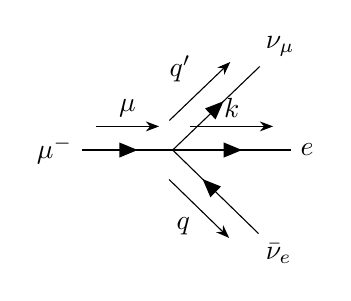
\begin{tikzpicture}
    \begin{feynman}
      \vertex (l) {$\mu^-$};
      \vertex [right=of l] (c);
      \vertex [above right=of c] (tr) {$\nu_\mu$};
      \vertex [right=of c] (r) {$e$};
      \vertex [below right=of c] (br) {$\bar{\nu}_e$};
      \diagram*{
        (l) -- [fermion, momentum=$\mu$] (c) -- [fermion, momentum=$k$] (r),
        (c) -- [anti fermion, momentum'=$q$] (br),
        (c) -- [fermion, momentum=$q'$] (tr),
      };
    \end{feynman}
  \end{tikzpicture}
\end{center}
We will assume neutrinos are massless.

The relevant bit of $\mathcal{L}_w^{\mathrm{eff}}$ is
\[
  - \frac{G_F}{\sqrt{2}} J^{\alpha\dagger}J_\alpha,
\]
where
\[
  J^\alpha = \bar{\nu}_e \gamma^\alpha (1 - \gamma^5) e + \bar{\nu}_\mu \gamma^\alpha(1 - \gamma^5)\mu + \bar{\nu}_\tau \gamma^\alpha(1 - \gamma^5) \tau.
\]
We see it is the interaction of the first two terms that will render this decay possible.

To make sure our weak field approximation is valid, we need to make sure we live in sufficiently low energy scales. For the decay to be possible, the most massive particle involved is
\[
  m_\mu \approx \SI{106}{\mega\electronvolt}.
\]
On the other hand, the mass of the weak boson is
\[
  m_W \approx \SI{80}{\mega\electronvolt}.
\]
We can now compute
\[
  M = \brak{e^-(k) \bar{\nu}_e (q) \nu_\mu(q')} \mathcal{L}_W^{\mathrm{eff}} \bket{\mu^-(p)}.
\]
Note that we left out all the spin indices to avoid overwhelming notation. We see that the first term in $J^\alpha$ is relevant to the electron bit, while the second is relevant to the muon bit. We can then write this as
\begin{align*}
  M &= -\frac{G_F}{\sqrt{2}} \brak{e^-(k) \bar{\nu}_e(q)} \bar{e} \gamma^\alpha (1 - \gamma^5) \nu_e \bket{0} \brak{\nu_\mu(q'} \bar{\nu}_\mu \gamma_\alpha(1 - \gamma^5) \mu \bket{\mu^-(p)}\\
  &= - \frac{G_F}{\sqrt{2}} \bar{u}_e(k) \gamma^\alpha (1 - \gamma^5)v_{\nu_e}(q) \bar{u}_{\nu_\mu} (q') \gamma_\alpha (1 - \gamma^5) u_p(p).
\end{align*}
Before we plunge through more computations, we look at what we are interested in and what we are not.

At this point, we are not interested in the final state spins. Therefore, we want to sum over the final state spins. We also don't know the initial spin of $\mu^-$. So we average over the initial states. So we want to look at
\begin{multline*}
  \frac{1}{2} \sum_{\mathrm{spins}} |M|^2 = \frac{1}{2} \frac{G_F^2}{2} \sum_{\mathrm{spins}} \left(\bar{u}_e(k) \gamma^\alpha (1 - \gamma^5) v_{\nu_e}(q) \bar{v}_{\nu_e}(q) \gamma^\beta (1 - \gamma^5) u_e(k)\right)\\
  \times \left(\bar{u}_{\nu_\mu} (q') \gamma_\alpha (1 - \gamma^5) u_\mu(p) \bar{u}_\mu (p) \gamma_\beta(1 - \gamma^5) u_{\nu_\mu}(q')\right).
\end{multline*}
We write this as
\[
  \frac{G_F^2}{4} S_1^{\alpha\beta}S_{2\alpha\beta},
\]
where the $S_1$ and $S_2$ are the two things in brackets.

To actually compute this, we need to use spinor identities etc, and after computation, we find
\begin{align*}
  S_1^{\alpha\beta} &= \Tr ((\slashed{k} + m_e) \gamma^\alpha (1 - \gamma^5) \slashed{q} \gamma^\beta(1 - \gamma^5))\\
  S_{2\alpha\beta} &= \Tr (\slashed{q}' \gamma_\alpha(1 - \gamma^5) (\slashed{p} + m_\mu) \gamma_\beta(1 - \gamma^5)).
\end{align*}
We can write this as
\begin{align*}
  S_1^{\alpha\beta} &= 8(k^\alpha q^\beta + k^\beta q^\alpha - k\cdot q g^{\alpha\beta} - i \varepsilon^{\alpha\beta\mu\rho} k_\mu q_\rho)\\
  S_{2\alpha\beta} &= 8(q'_\alpha p_\beta + q'_\beta p_\alpha - q' \cdot p g_{\alpha\beta} - i \varepsilon_{\alpha\beta\mu\rho} q'^\mu p^\rho
\end{align*}
This leads to the much more pleasant result
\[
  \frac{1}{2} \sum |M|^2 = 64 G_F^2 (p \cdot q)(k \cdot q').
\]
To understand this, consider the case where $e^-$ and $\nu_\mu$ go out along the $+z$ and $\bar{\nu}_e$ along $-z$. Then we have
\[
  k \cdot q' = \sqrt{m_e^2 + k_z^2} q_z' - k_z q'_z.
\]
This $\to 0$ if $m_e \to 0$. This makes sense, because the weak interaction couples to left-handed chiral particles and right-handed anti-particles.
\begin{center}
  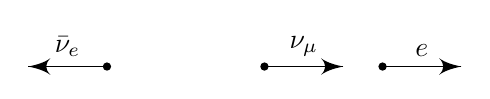
\begin{tikzpicture}
    \node [circ] {};
    \draw [->] (0, 0) -- (-1, 0) node [pos=0.5, above] {$\bar{\nu}_e$};

    \node [circ] at (2, 0) {};
    \draw [->] (2, 0) -- (3, 0) node [pos=0.5, above] {$\nu_\mu$};

    \node [circ] at (3.5, 0) {};
    \draw [->] (3.5, 0) -- (4.5, 0) node [pos=0.5, above] {$e$};
  \end{tikzpicture}
\end{center}
Thus, the spin of $\bar{\nu}_e$ must be opposite to that of $\nu_\mu$ and $e^-$. So they all point in the same direction, and the total spin would be $\frac{3}{2}$, which exceeds the initial spin $\frac{1}{2}$, and this violates conservation of angular momentum.

But if $m_e \not= 0$, then the left-handed and right-handed components of the electron are coupled, and helicity and chirality do not coincide. So it is possible that we obtain a right-handed electron instead, and this gives conserved angular momentum. We call this \term{helicity suppression}. Note that this is the case only when the electrons and neutrinos move in theses particular directions. If $m_e = 0$, we can still have decays in other directions.

We can now compute the decay rate,
\begin{multline*}
  \Gamma = \frac{1}{2 m_\mu} \int \frac{\d^3 k}{(2\pi)^3 2k^0} \int \frac{\d^3 q}{(2\pi)^3 2q^0} \int \frac{\d^3 q'}{(2\pi)^3 q'^0} \\
  \times (2\pi)^4 \delta^{(4)}(p - k - q - q') \frac{1}{2} \sum |M|^2.
\end{multline*}
Using our expression for $|M|$, we find
\[
  \Gamma = \frac{G_F^2}{8 \pi^5 m_\mu} \int \frac{\d^3 k\; \d^3 q\; \d^3 q'}{k^0 q^0 q'^0} \delta^{(4)} (p - k - q - q') (p \cdot q) (k \cdot q').
\]
To evaluate this integral, there is a useful trick.

Consider
\[
  I_{\mu\nu}(p - k) = \int \frac{\d^3 q}{q^0} \frac{\d^3 q'}{q'^0} \delta^{(4)}(p - k - q - q') q_\mu q'_\nu.
\]
By Lorentz symmetry arguments, this must be of the form
\[
  I_{\mu\nu} (p - k) = a((p - k)^2) (p - k)_\mu (p - k)_\nu + b((p - k)^2) g_{\mu\nu} (p - k)^2,
\]
where $a, b: \R \to \R$ are some scalar functions.

Now consider
\[
  g^{\mu\nu} I_{\mu\nu} = \int \frac{\d^3 q}{q^0} \frac{\d^3 q'}{q'^0} \delta^{(4)}(p - k - q - q') q \cdot q' = (a + 4b) (p - k)^2 .
\]
But we also know that
\[
  (q + q')^2 = q^2 + q'^2 + 2 q \cdot q' = 2 q \cdot q'
\]
because neutrinos are massless. On the other hand, by momentum conservation, we know
\[
  q + q' = p - k.
\]
So we know
\[
  q \cdot q' = \frac{1}{2} (p - k)^2.
\]
So we find that
\[
  a + 4b = \frac{I}{2},\tag{$1$}
\]
where
\[
  I = \int \frac{\d^3 q}{q^0} \int \frac{\d^3 q'}{q'^0} \delta^{(4)} (p - k - q - q').
\]
To evaluate this integral, we can, for example, just evaluate it in a frame where $p - k = 0$, so that $q = q'$. % insert value of integral.

We can consider something else. We have
\[
  (p - k)^\mu (p - k)^\nu I_{\mu\nu} = a(p - k)^4 + b(p - k)^4 = \int \frac{\d^3 q}{q^0} \int \frac{\d^3 q'}{q'^0} \delta^{(4)} (p - k - q - q') q\cdot (p - k) \cdot q' (p - k).
\]
Using the masslessness of neutrinos and momentum conservation again, we find that
\[
  q \cdot (p - k) q \cdot (p - k) = (q \cdot q') (q \cdot q').
\]
So we find
\[
  a + b = \frac{I}{4}\tag{$2$}.
\]
So we find that
\[
  \Gamma = \frac{G_F^2}{(2\pi)^4 3m_\mu} \int \frac{\d^3 k}{k^0} \left(2 p \cdot (p - k) k \cdot (p - k) + (p \cdot k)(p - k)^2\right)
\]
Recall that we are working in the reset frame of $\mu$. So we know that $p \cdot k = m_\mu E$. Then we have
\[
  p \cdot k = m_\mu E,\quad p \cdot p = m_\mu^2,\quad k \cdot k = m_e^2,
\]
where $E = k^0$. Note that we have
\[
  \frac{m_\mu}{m_e}\approx 0.0048 \ll 1.
\]
So to make our lives easier, it is reasonable to assume $m_e = 0$. So we have
\begin{align*}
  \Gamma &= \frac{G_F^2}{(2\pi)^4 3m_\mu} \int \frac{\d^3 k}{E} \Big(2 m_\mu^2 m_\mu E - 2 (m_\mu E)^2 - 2 (m_\mu E)^2 + m_\mu E m_\mu^2\Big)\\
  &= \frac{G_F^2 m_\mu}{ (2\pi)^4 3} \int \d^3 k\; (3 m_\mu - 4 E)\\
  &= \frac{4\pi G_F^2 m_\mu}{(2\pi)^4 3} \int \d E\; E^2(3 m_\mu - 4E)
\end{align*}
Here we are using the fact (or approximation) that the mass of the electron is $0$, so we have $|\mathbf{k}| = E$.

We now need to figure out what we want to integrate over. When $e$ is at rest, then $E_{\mathrm{min}} = 0$. The maximum energy is obtained when $\nu_\mu, \bar{\nu}_e$ are in the same direction and opposite to $e^-$. In this case, we have
\[
  E + (E_{\bar{\nu}_e} + E_{\nu_\mu}) = m_\mu.
\]
By energy conservation, we also have
\[
  E - (E_{\bar{\nu}_e} + E_{\nu_\mu}) = 0.
\]
So we find
\[
  E_{\mathrm{max}} = \frac{m_\mu}{2}.
\]
Thus, we can put in our limits into the integral, and find that % figure out where the limits come from.
\[
  \Gamma = \frac{G_F^2 m_\mu^5}{192 \pi^3}.
\]
As we mentioned at the beginning of the chapter, this is the only decay channel off the muon. From experiments, we can measure the lifetime of the muon as
\[
  \tau_{\mu} = \SI{2.1870e-6}{\second}.
\]
This tells us that
\[
  G_F = \SI{1.164e-5}{\giga\electronvolt\squared}.
\]
Of course, this isn't quite right, because we ignored all loop corrections (and approximated $m_e = 0$). But this is reasonably good, because those effects are very small, at an order of $10^{-6}$ as large. Of course, if we want to do more accurate and possibly beyond standard model physics, we need to do better than this.

Experimentally, $G_F$ is consistent with what we find in the $\tau \to e \bar{\nu}_e \nu_\tau$ and $\mu \to e \bar{\nu}_e \nu_\mu$ decays. This is some good evidence for lepton universality, ie. they have different masses, but they couple in the same way.

We go back to the set up where $e, \bar{\nu}_e, \nu_\mu$ are along the positive and negative $z$ axis. We assume $m_e \not= 0$.
\begin{center}
  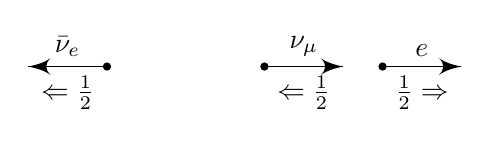
\begin{tikzpicture}
    \node [circ] {};
    \draw [->] (0, 0) -- (-1, 0) node [pos=0.5, above] {$\bar{\nu}_e$} node [pos=0.5, below] {$\Leftarrow \frac{1}{2}$};

    \node [circ] at (2, 0) {};
    \draw [->] (2, 0) -- (3, 0) node [pos=0.5, above] {$\nu_\mu$} node [pos=0.5, below] {$\Leftarrow \frac{1}{2}$};

    \node [circ] at (3.5, 0) {};
    \draw [->] (3.5, 0) -- (4.5, 0) node [pos=0.5, above] {$e$} node [pos=0.5, below] {$\frac{1}{2} \Rightarrow$};
  \end{tikzpicture}
\end{center}
Under partiy transform, the momenta reverse, but spins don't. If we transform under parity, we would expect to see the same behaviour.
\begin{center}
  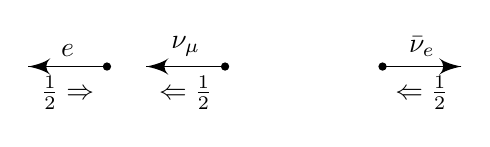
\begin{tikzpicture}[xscale=-1]
    \node [circ] {};
    \draw [->] (0, 0) -- (-1, 0) node [pos=0.5, above] {$\bar{\nu}_e$} node [pos=0.5, below] {$\Leftarrow \frac{1}{2}$};

    \node [circ] at (2, 0) {};
    \draw [->] (2, 0) -- (3, 0) node [pos=0.5, above] {$\nu_\mu$} node [pos=0.5, below] {$\Leftarrow \frac{1}{2}$};

    \node [circ] at (3.5, 0) {};
    \draw [->] (3.5, 0) -- (4.5, 0) node [pos=0.5, above] {$e$} node [pos=0.5, below] {$\frac{1}{2} \Rightarrow$};
  \end{tikzpicture}
\end{center}
But (at least in the limit of masslessneutrinos) this isn't allowed, because weak interactions don't couple to right-handed neutrinos. So we know that weak decays violate P.

\subsection{Pion decay}
We are now going to look at a slightly different example, which is simpler in some sense, and more complicated in some other sense. This is simpler, because there are less particles involved, but more complicated because there are quarks. We are looking at
\[
  \pi^- (\bar u d) \to e^- \bar{\nu}_e.
\]
\begin{center}
  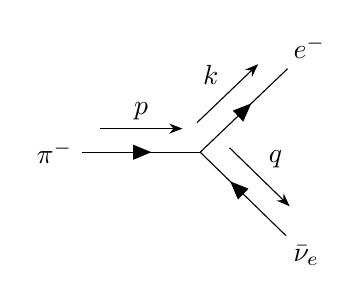
\begin{tikzpicture}
    \begin{feynman}
      \vertex (c);
      \vertex [left=of c] (pi) {$\pi^-$};
      \vertex [above right=of c] (e) {$e^-$};
      \vertex [below right=of c] (nu) {$\bar{\nu}_e$};

      \diagram*{
        (pi) -- [fermion, momentum=$p$] (c) -- [fermion, momentum=$k$] (e);
        (c) -- [anti fermion, momentum=$q$] (nu);
      };
    \end{feynman}
  \end{tikzpicture}
\end{center}
The $\pi^-$ is made up of $d$ and $\bar{u}$ quarks, but they do not propagate freely. They are bound inside $\pi^-$.

The relevant currents are
\begin{align*}
  J_{\mathrm{lept}}^\alpha &= \bar{\nu}_e \gamma^\alpha (1 - \gamma^5) e\\
  J_{\mathrm{had}}^\alpha &= \bar{u} \gamma^\alpha (1 - \gamma^5)(v_{ud} d + \cdots) \equiv V_{\mathrm{had}}^\alpha - A_{\mathrm{had}}^\alpha,
\end{align*}
Where the $V_{\mathrm{had}}^\alpha$ contains the $\gamma^\alpha$ bit, while $A_{\mathrm{had}}^\alpha$ contains the $\gamma^\alpha \gamma^5$ bit.

The amplitude is
\begin{align*}
  M &= \brak{e^-(k) \bar{\nu}_e (q)} \mathcal{L}_W^{\mathrm{eff}} \bket{\pi^-(p)}\\
  &= - \frac{G_F}{\sqrt{2}} \brak{e^-(k) \bar{\nu}_e(q)} \bar{e} \gamma_\alpha (1 - \gamma^5) \nu_e \bket{0} \brak{0} J_{\mathrm{had}}^\alpha \bket{\pi^-(p)}\\
  &= \frac{G_F}{\sqrt{2}} \bar{u}_e (k) \gamma_\alpha(1 - \gamma^5) v_{\nu_e}(q) \brak{0} V_{\mathrm{had}}^\alpha - A_{\mathrm{had}}^\alpha \bket{\pi^-(p)}.
\end{align*}
We now note that $V_{\mathrm{had}}^\alpha$ does not contribute, because QCD is P-invariant, and $\pi$ has spin $0$ and negative parity. If we look at $\brak{0}\bar{u} \gamma^\alpha d \bket{\pi^-(p)}$, then we find that $\bar{u} \gamma^\alpha d$ and $\bket{\pi^-(p)}$ transform differently, and we can show that it is equal to the negative of itself. Since we don't do physics over characteristic $2$, it follows that it must vanish.

We parameterize the unknown non-perturbative QCD part in the pion decay constant, $F_\pi$, defined by
\[
  \brak{0} \bar{u} \gamma^\alpha \gamma^5 d \brak{\pi^-(p)} = i \sqrt{2} F_\pi p^\alpha.
\]
Then we have
\[
  M = i G_F F_\pi V_{ud} \bar{u}_e(k) \slashed p (1 - \gamma^5) v_{\nu_e}(q).
\]
Using the fact that $p = k + q$, and using spinor identities, we find
\[
  M = i G_F F_\pi V_{ud} m_e \bar{u}_e(k) (1 - \gamma^5) v_{\nu_e}(q).
\]
If we want to calculate the decay rate, we need to integrate and add over this $M$. In particular, we need to average over all spins. Since the initial state is spinless, we don't have to average over the initial spins.

We have
\begin{align*}
  \sum_{\text{spins }e, \bar{\nu}_e} |M|^2 &= \sum_{\mathrm{spins}} |G_F F_\pi m_e V_{ud}|^2 [\bar{u}_e(k) (1 - \gamma^5) v_{\nu_e}(q) \bar{v}_{\nu_e}(q) (1 + \gamma^5) u_e(k)]\\
  &= 8 |G_F F_\pi m_e V_{ud}|^2 (k \cdot q.
\end{align*}
This again shows helicity suppression. The spin-$0$ $\pi^-$ decays to the positive helicity $\bar{\nu}_e$, and hence decays to a positive helicity electron by helicity conservation.
\begin{center}
  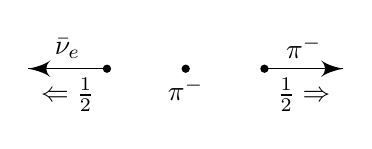
\begin{tikzpicture}
    \node [circ] {};
    \node [below] at (0, 0) {$\pi^-$};

    \draw [->] (1, 0) node [circ] {} -- (2, 0) node [pos=0.5, above] {$\pi^-$} node [pos=0.5, below] {$\frac{1}{2} \Rightarrow$};
    \draw [->] (-1, 0) node [circ] {} -- (-2, 0) node [pos=0.5, above] {$\bar{\nu}_e$} node [pos=0.5, below] {$\Leftarrow \frac{1}{2}$};
  \end{tikzpicture}
\end{center}
But if $m_e = 0$, then this has right-handed chirality, and so this decay is forbidden. This is again a scenario that is impossible if we have zero electron mass.

We can now compute
\begin{align*}
  \Gamma_{\pi \to e \bar{\nu}_e} &= \frac{1}{2 m_\pi} \int \frac{\d^3 k}{(2\pi)^3 2 k^0} \int \frac{\d^3 q}{(2\pi)^3 2 q^0} (2\pi)^4 \delta^{(4)}(p - k - q) 8 |G_F F_\pi m_e V_{ud}|^2 (k \cdot q)\\
  &= \frac{|G_F F_\pi m_e V_{ud}|^2 }{4 m_\pi \pi^2} \int \frac{\d^3 k}{(2\pi)^3 2 k^0} \delta(m_{\pi} - E - |\mathbf{k}|) (E |\mathbf{k}| + |\mathbf{k}|^2)\\
  \intertext{where $E = k^0$ is the energy of $e^-$, and since the electron is massless, we have $q^0 = |\mathbf{q}| = |\mathbf{k}|$}
  &= \frac{|G_F F_\pi m_e V_{ud}|^2}{4 \pi^2 m_\pi}\int \frac{4\pi k^2 \;\d k}{E} \frac{E + k}{1 + k_0/E} \delta(k - k_0)\\
  \intertext{where $k_0 = \frac{m_\pi^2 - m_e^2}{2 m_\pi}$}
  &= \frac{|G_F F_\pi V_{ud}|^2}{4\pi} m_e^2 m_\pi \left(1 - \frac{m_e^2}{m_\pi^2}\right)^2.
\end{align*}
Note that if we set $m_e \to 0$, then this vanishes. This time, it is the whole decay rate, and not just some particular decay channel.

Let's try to match this with experiment. Instead of looking at the actual lifetime, we compare it with some other possible decay rates. The expression for $\Gamma_{\pi \to \mu \bar{\nu}_\mu}$ is exactly the same, with $m_e$ replaced with $m_\mu$. So the ratio
\[
  \frac{\Gamma_{\pi \to e\bar{\nu}_e}}{\Gamma_{\pi \to \mu \bar{\nu}_\mu}} = \frac{m_e^2}{m_\mu^2} \left(\frac{m_\pi^2 - m_e^2}{m_\pi^2 - m_\mu^2}\right)^2 \approx 1.28 \times 10^{-4}.
\]
Here all the decay constants cancel out. So we can actually compare this with experiment just by knowing the electron and muon masses. When we actually do experiments, we find $1.230(4) \times 10^{-4}$. This is pretty good agreement, but not agreement to within experimental error. Of course, this is not unexpected, because we didn't include the quantum loop effects in our calculations.

Another thing we can see is that the ration is very small, on the order of $10^{-4}$. This we can understand from helicity suppression, because $m_\mu \gg m_e$, so the helicity suppression is less.

Note that we were able to get away without knowing how QCD works!

\subsection{\texorpdfstring{$K^0\mdash \bar{K}^0$}{K0-K0} mixing}
We now look at our third example of weak decays --- $K^0 \mdash \bar{K}^0$ mixing. \term{Kaons} contain a strange quark/antiquark. The ``flavour eigenstates'' are
\[
  K^0  (\bar{s} d),\quad \bar{K}^0  (\bar{d} s),\quad K^+(\bar{s} u),\quad K^-(\bar{u} s).
\]
These are the lightest kaons, and they have spin $J = 0$ and parity $p = -$, and we write this as $J^p = 0^-$. These are ``pseudoscalars''.

For kaons at rest, we can pick the relative phases such that
\[
  \hat{C} \hat{P} \bket{K^0} = - \bket{\bar{K}^0}.
\]
here we are just fixing the constant factor behind $\bket{\bar{K}^0}$ to be $-$. Similarly, we have
\[
  \hat{C} \hat{P} \bket{\bar{K}^0} = - \bket{K^0}.
\]
So the CP eigenstates are just
\[
  \bket{K_\pm^0} = \frac{1}{\sqrt{2}} (\bket{K^0} \mp \bket{\bar{K}^0}).
\]
Then we have
\[
  \hat{C}\hat{P} \bket{K_{\pm}^0} = \pm \bket{K_{\pm}^)}.
\]
Let's consider the decays $K^0 \to \pi^0 \pi^0$ and $K^0 \to \pi^+ \pi^-$. This requires converting one of the strange quarks into an up or down quark.
%\begin{center}
%  \begin{tikzpicture}
%    \begin{feynman}
%      \vertex (tl) {$d$};
%      \vertex [below=of tl] (bl) {$\bar{s}$};
%      \vertex  [right=of bl] (c);
%      \vertex [right=of c] (br) {$\bar{u}$};
%      \vertex [above=of br] (tr);
%
%      \vertex [below=of c] {$W^+$};
%      \vertex [right=of c] {$u$};
%      \vertex [below right=of c]{$\bar{d}$};
%    \end{feynman}
%  \end{tikzpicture}
%\end{center}
% insert a picture!

From the conservation of angular momentum, the total angular momentum of $\pi \pi$ is zero. Since they are also spinless, the orbital angular momentum $L = 0$.

Recall that the parity affects angular momentum by
\[
  \hat{C}\hat{P} \bket{\pi^+\pi^-} = (-1)^L \bket{\pi^+\pi^-} = \bket{\pi^+ \pi^-},
\]
where the relative phases of $\pi^+$ and $\pi^-$ cancel out. Similarly, we have
\[
  \hat{C}\hat{P} \bket{\pi^0 \pi^0} = \bket{\pi^0 \pi^0}.
\]
Therefore $\pi \pi$ is always a CP eigenstate with eigenvalue $+1$.

Since $\hat{C}\hat{P}$ is conserved by strong and electromagnetic interactions, if it is conserved by the weak interactions as well, then the mass eigenstates would be $\bket{K_{\pm}^0}$, and $K^0_+ \to \pi \pi$ is permitted. So $K^0_+$ is a ``short-lived'' state. On the other hand, $K_-^0 \to \pi \pi$ is impossible! So it must decay in ways like $K_-^0 \to \pi \pi \pi$, or other final states, and $K_-^0$ is ``long-lived''.

In experiments, we found a Kaon $K^0_S$  has ``short'' lifetime, with $\tau \approx \SI{9e-11}{\second}$, and a  ``long--lived'' Kaon $K_L^0$ has $\tau \approx \SI{5e-8}{\second}$.

But this doesn't immediately verify that CP is conserved. We want to see if $K_L^0$ can decay to $\pi \pi$ or not. We define
\begin{align*}
  \eta_{+ -} &= \frac{|\brak{\pi^+ \pi^-}H \bket{K_L^0}|}{|\brak{\pi^+ \pi^-}H \bket{K_L^0}|}\\
  \eta_{0 0} &= \frac{|\brak{\pi^0 \pi^0}H \bket{K_L^0}|}{|\brak{\pi^0 \pi^0}H \bket{K_L^0}|}
\end{align*}
Experimentally, when we measure these things, we have
\[
  \eta_{\pm} \approx \eta_{00} \approx 2.2\times 10^{-3} \not= 0.
\]
This tells us we have CP violation.

If we think about what is going on here, there are two ways CP can be violated:
\begin{itemize}
  \item Direct CP violation of $s \to u$ due to a phase in $V_{CKM}$.
  \item Indirect CP violation due to $K^0 \to \bar{K}^0$ or vice-versa, then decaying.
\end{itemize}
Of course, ultimately, the ``indirect violation'' is still due to phases in the CKM matrix, but the second is more ``higher level''.

It turns out in this particular process, it is the indirect CP violation that is mainly responsible, and the dominant contributions are ``box diagrams'', where the change in strangeness $\Delta S = 2$.
\begin{center}
  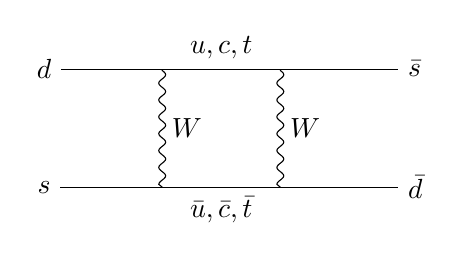
\begin{tikzpicture}
    \begin{feynman}
      \vertex (ull) {$d$};
      \vertex (ul) [right=of ull];
      \vertex (ur) [right=of ul];
      \vertex (urr) [right=of ur] {$\bar{s}$};

      \vertex (dll) [below= of ull] {$s$};
      \vertex (dl) [right=of dll];
      \vertex (dr) [right=of dl];
      \vertex (drr) [right=of dr] {$\bar{d}$};

      \diagram*{ % label middle one as u, c, t on top and \bar{*} below
      (ull) -- (ul) -- [edge label={$u, c, t$}] (ur) -- (urr),
      (dll) -- (dl) -- [edge label'={$\bar{u}, \bar{c}, \bar{t}$}] (dr) -- (drr),
      (ul) -- [photon, edge label=$W$] (dl),
      (ur) -- [photon, edge label=$W$] (dr), % label as W, for both
    };
  \end{feynman}
  \end{tikzpicture}
\end{center}
and
\begin{center}
  \begin{tikzpicture}
    \begin{feynman}
      \vertex (ull) {$d$};
      \vertex (ul) [right=of ull];
      \vertex (ur) [right=of ul];
      \vertex (urr) [right=of ur] {$\bar{s}$};

      \vertex (dll) [below= of ull] {$s$};
      \vertex (dl) [right=of dll];
      \vertex (dr) [right=of dl];
      \vertex (drr) [right=of dr] {$\bar{d}$};

      \diagram*{ % label middle one as u, c, t on top and \bar{*} below
      (ull) -- (ul) -- (dl) -- (dll),
      (urr) -- (ur) -- (dr) -- (drr),
      (ul) -- [photon] (ur),
      (dl) -- [photon] (dr), 
    };
  \end{feynman}
  \end{tikzpicture}
\end{center}
This is next-to-leading order in perturbation theory. We find that
\begin{align*}
  \bket{K_S^0} &= \frac{1}{\sqrt{1 + |\varepsilon_1|^2}} (\bket{K_+^0} + \varepsilon_1 \bket{K_-^0}) \approx \bket{K_+^0}\\
  \bket{K_L^0} &= \frac{1}{\sqrt{1 + |\varepsilon_2|^2}} (\bket{K_0^0} + \varepsilon_2 \bket{K_+^0}) \approx \bket{K_-^0},
\end{align*}
where $\varepsilon_1, \varepsilon_2 \in \C$ are some small complex numbers.

We assume that we just have two state mixing, and ignore details of the strong interaction. Then as time progresses, we have
\begin{align*}
  \bket{K_S(t)} &= a_S(t) \bket{K^0} + b_S(t) \bket{\bar{K}^0}\\
  \bket{K_L(t)} &= a_L(t) \bket{K^0} + b_L(t) \bket{\bar{K}^0}
\end{align*}
for some (complex) functions $a_S, b_S, a_L, b_L$. Then by Schr\"odinger's equation, we have
\[
  i \frac{\d}{\d t} \bket{\psi(t)} = H \bket{\psi(t)}.
\]
So we have
\[
  i \frac{\d}{\d t}
  \begin{pmatrix}
    a\\ b
  \end{pmatrix} =
  R
  \begin{pmatrix}
    a\\b
  \end{pmatrix},
\]
where
\[
  R = 
  \begin{pmatrix}
    \brak{K^0}H' \bket{K^0} & \brak{K^0}H' \bket{\bar{K}^0}\\
    \brak{\bar{K}^0}H' \bket{K^0} & \brak{\bar{K}^0}H' \bket{\bar{K}^0}
  \end{pmatrix}
\]
where $H'$ is the next-to-leading order weak Hamiltonian. Because Kaons decay, $R$ is not Hermitian. We can write it as
\[
  R = M - \frac{i}{2} \Gamma,
\]
where $M$ is the mass matrix, and $\Gamma$ is the decay matrix, and both are Hermitian.

We are not going to actually compute $R$, but we are going to use the known symmetries to put some constraint on $R$. If $\Theta =  \hat{C}\hat{P}\hat{T}$,  then by the CPT theorem, we have
\[
  \Theta H' \Theta^{-1} = H'^\dagger. % why dagger?
\]
In the rest frame of a particle $\bar{K}^0$, we have
\[
  \Theta \bket{\bar{K}^0} = - \bket{K^0},\quad \Theta \bket{K^0} = - \bket{\bar{K}^0},
\]
since we know that $\hat{T} \bket{K^0} = \bket{K^0}$, and similarly for $\bar{K}^0$.

Since we are going to involve time reversal, we stop using bra-ket notation for the moment. We have
\begin{align*}
  R_{11} &= (K^0, H' K^0) \\
  &= (\Theta^{-1}\Theta K^0,  H' \Theta^{-1}\Theta K^0)\\
  &= (\bar{K}^0, H'^\dagger \bar{K}^0)^*\\
  &= (H' \bar{K}^0, \bar{K}^0)^*\\
  &= (\bar K^0, h' \bar{K}^0)\\
  &= R_{22}
\end{align*}
Now \emph{if} $\hat{T}$ was a good symmetry (ie. $\hat{C}\hat{P}$ is good as well), ten a similar computation shows that
\[
  R_{12} = R_{21}.
\]
We can show that we in fact have
\[
  \varepsilon_1 = \varepsilon_2 = \varepsilon = \frac{\sqrt{R_{21}} - \sqrt{R_{21}}}{\sqrt{R_{12}} + \sqrt{R_{21}}}.
\]
So if CP is conserved, then $R_{12} = R_{21}$, and therefore $\varepsilon_1 = \varepsilon_2 = \varepsilon = 0$.

But if $R_{12}$ and $R_{21}$ are different, which requires CP violation, then we can indeed have mixing.

One can also show that We can also show that
\[
  \eta_{+-} = \varepsilon + \varepsilon',\quad \eta_{00} = \varepsilon - 2 \varepsilon',
\]
where $\varepsilon'$ measures the direct source of CP violation. By looking at these two modes of decay, we can figure out the values of $\varepsilon$ and $\varepsilon'$. Experimentally, we find
\[
  |\varepsilon| = (2.228 \pm 0.011) \times 10^{-3},
\]
and
\[
  \left|\frac{\varepsilon}{\varepsilon'}\right| = (1.66 \pm 0.23) \times 10^{-3}.
\]
As claimed, it is the indirect CP violation that is dominant, and the direct one is suppressed by a factor of $10^{-3}$.

Other decays can be used to probe $K_{L, S}^0$. For example, we can look at semi-leptonic decays
\[
  K^0 \to \pi^- e^+ \nu_e.
\]
One can show that we cannot have
\[
  K^0 \to \pi^+ e^- \bar{\nu}_e,
\]
while the $\bar{K}^0$ has the opposite phenomenon.

To show these, we just have to try to write down diagrams for these events. % insert diagram

Now if CP is conserved, we'd expect the decay rates
\[
  \Gamma(K_{L, S}^0 \to \pi^- e^+  \nu_e) = \Gamma(K_{L, S}^0 \to \pi^+ e^- \bar{\nu}_e),
\]
since we expect $K_{L, S}$ to consist of the same amount of $K^0$ and $\bar{K}^0$.

We define
\[
  A_L = \frac{\Gamma(K_L^0 \to \pi^- e^+ \nu_e) - \Gamma(K_L^0 \to \pi^+ e^- \bar{\nu}_e)}{\Gamma(K_L^0 \to \pi^- e^+ \nu_e) + \Gamma(K_L^0 \to \pi^+ e^- \bar{\nu}_e)}.
\]
If this is non-zero, then we have evidence for CP violation. Experimentally, we find
\[
  A_L = (3.32 \pm 0.06) \times 10^{-3} \approx 2 \Re (\varepsilon).
\]
This is small, but certainly significantly non-zero.

We can actually use CP violation to tell some aliens far far away what we mean by matter and anti-matter. % include

\section{Quantum chromodynamics (QCD)}
Historically, the idea of quarks grew out of studying multiplets with similar properties. People grouped things together based on similarities, and tried to understand them, and eventually the idea of QCD came out.

We find protons and neutrons have similar masses, and so do the pions $\pi^+, \pi^-$ and $\pi^0$. This lead to the idea of an $\SU(2)_I$ symmetry, a (global) \term{isospin symmetry}. 

\printindex
\end{document}
